
\chapter{Addressing Serialization Errors by Discarding Sequential Position Information}
\label{chapter:layout2pos}

\renewcommand{\leftmark}{\spacedlowsmallcaps{Addressing Serialization Errors by Discarding Sequential Position Information}}

\begin{chapabstract}
    {\em
    Chapter Abstract


    \vspace*{5mm}
    The work in this chapter has led to the submission of a paper currently under review:}
    \begin{itemize}
        \item \small \fullcite{}.
    \end{itemize}
\end{chapabstract}

\ifthenelse{\boolean{skipCh7}}{\endinput}{}


\newpage

\minitoc
\chapterwithfigures{\nameref*{chapter:layout2pos}}
\chapterwithtables{\nameref*{chapter:layout2pos}}

% Textual content is organized in a specific layout to convey meaning and context. Layout holds considerable importance in conveying information, whether in business documents, scholarly papers, news articles or other written materials. 

The organization of textual content in a specific layout is crucial for conveying meaning and context, holding significant importance across various written materials, including business documents, scholarly papers, and news articles. In particular, layout determines the sequence in which text is intended to be read or processed within a document, \textit{i.e.}, the \textit{reading order}. A well-designed reading order ensures that readers can follow the logical flow and structure of information and comprehend the intended meaning of the text. However, defining a proper reading order is non-trivial due to the complexity of document layouts, which may include elements such as tables and multiple columns.

% Hence, reading order is crucial for models to perform well because it reflects the natural flow and structure of information in a document. 
When models are trained with a reading order that aligns with human understanding, they learn to capture the relationships between words, sentences, and paragraphs. Hence, reading order is crucial for models to perform well. Most pre-training methods for Document Understanding rely on serialized text, where either an \ac{OCR} engine or a PDF parser is used to extract text. However, due to the variety of layout formats, most \ac{OCR} engines and PDF parsers struggle to provide accurate reading orders, introducing \textit{serialization errors}. Serialization errors, \textit{i.e.}, noise that may arise during text extraction, such as misinterpretations or omissions, can lead to misalignments between the extracted text and the original visual content. For instance, an \ac{OCR} engine might misinterpret or introduce extraneous characters, while a PDF parser might misinterpret formatting elements or misorder words. 

Most of the time, the text extracted is re-arranged in a raster-scan order, aligning tokens from the top-left to the bottom-right corner \citep{clausner2013significance}. However, this linear organization does not always align with human reading patterns, particularly in documents with complex layouts such as multicolumn texts, tables, and forms. Serialization errors impact the accuracy of the extracted text and, therefore, affect the entire text processing pipeline. Without an accurate reading order, models may misinterpret the relationships between different parts of the text, resulting in suboptimal performance in downstream tasks. This poses a substantial challenge in various applications, notably in the field of Document Understanding, where document layouts can be complex. 

Furthermore, in real-word scenarios, documents may be processed by various \ac{OCR} engines for different reasons such as cost, availability, or integration with existing workflows. Each \ac{OCR} engine may have unique characteristics related to layout, font handling, or language support. These differences can introduce variations in the quality and accuracy of the \ac{OCR} output for the same document, impacting, most importantly, the reading order. This variability may result in significant fluctuations in downstream performance. However, it is crucial for organizations to be able to choose \ac{OCR} engines based on their specific requirements without compromising performance in downstream tasks.

% Furthermore, inaccuracies in \ac{OCR} outputs often require manual correction, which can be time-consuming and resource-intensive.

In particular, in visual information extraction tasks, where the goal is to recognize word sequences in a document as entities of predefined semantic types (\textit{e.g.}, names, dates, addresses), performance is significantly affected by serialization errors. Following the classic settings of \ac{NLP}, the task is commonly framed as a sequence-labeling problem. This approach involves labeling each token using a tagging scheme, such as BIO-tagging \citep{ramshaw1999text}, and leveraging these tags to identify entities. A sequence labeling-based approach operates under the assumption that each identified segment of an entity forms a continuous sequence of words within the input. While this assumption is valid for plain texts, it may not hold for real-world documents, where \ac{OCR} systems or PDF parsers might not correctly recognize and organize text. For instance, an entity might be split into non-continuous fragments. Such disordered input disrupts the BIO-tagging scheme, preventing the models from accurately identifying entities.

On the other hand, layout inherently encapsulates the correct reading order of documents by visually organizing content in a structured manner. A well-designed layout guides the reader's natural progression from one section to another, ensuring coherent and logical information flow. Therefore, understanding the layout provides essential cues for determining the correct reading order, as it aligns with the visual hierarchy and structure intended by document creators. 

Yet, existing pre-training methods for Document Understanding often neglect this aspect, opting to oversimply the integration of layout. For instance, LayoutLM \citep{XYLayoutLM} incorporates layout information as an extra embedding in the input layer, while LayoutLMv2 \citep{xu2020layoutlmv2} adds it as a bias term in the attention layer. Although ERNIE-Layout \citep{peng2022ernie} learns the relationship between layout and reading order through a pre-training strategy involving reading order prediction, it continues to rely on sequential position embeddings derived from the reading order obtained via \ac{OCR}. However, by investigating the position-awareness in causal language models with no explicit positional encodings, \citet{haviv2022transformer} show that these models develop an implicit understanding of absolute positions to compensate for missing information. It is suggested that causal attention, a mechanism in which each token attends only to its preceding positions in a sequence, allows the model to estimate the number of predecessors each token can attend to, thereby approximating its absolute position. Our objective is to demonstrate that the capability of a model to approximate its absolute position is not restricted to causal models, but holds true across various scenarios when layout information is provided.

Unlike the sequence labeling approach that entirely depends on the sequential arrangement of information, generative models, particularly those based on transformers, generate content in a manner that is not bound by the document's original order.

% In particular, Visual Information Extraction heavily relies on the detected text and reading order provided by \ac{OCR}. Inaccuracies in the reading order can disrupt the structure of the extracted data, leading to issues such as entities being split into non-contiguous fragments. Besides, the task is commonly framed as a sequence labeling task, and common labeling schemes used to annotate entities in a sequence for sequence labeling, such as the BIO-tagging scheme \citep{ramshaw1999text}, entirely depend on the detected reading order. Furthermore, in the context of sequence labeling, the model's output is restricted to the detected words. As a consequence, there might be no exact match for the expected value in a document. 

In this chapter, we focus on mitigating serialization errors by \textit{entirely discarding sequential position information}. We introduce \textit{Layout2Pos}, a shallow Transformer model designed to generate 1D position embeddings from the document layout by learning to reconstruct the relative order between tokens. Our endeavor is twofold: from a practical standpoint, we aim to enhance the robustness of models to reading order changes, crucial for real-world applications; from a theoretical perspective, we demonstrate that it is feasible to discard sequential position information without compromising overall performance. Following specific pre-training designed to instill the model with the ability to learn the reading order from layout information, we incorporate this module into sequence-to-sequence models for visual information extraction tasks. This integration eliminates the reliance on reading order and enables the generation of values that are not explicitly present in the input during entity extraction.


\section{Reconstructing Positional Information from 2D Positions}

In this section, we present preliminary experiments that underscore the limitations inherent in OCR outputs in terms of accurately preserving the reading order of tokens. In response to the challenges posed by OCR-induced serialization errors, we introduce a novel approach named Layout2Pos. This module goes beyond conventional approaches by discarding the reliance on reading order information. Instead, Layout2Pos leverages the inherent 2D positional information of tokens within the document page to reconstruct sequential positional information, thereby enhancing the robustness and reliability of downstream tasks.

\subsection{Preliminary Experiments: OCR Serialization Errors}

To gauge the extent of \ac{OCR}-induced serialization errors, we conduct preliminary experiments comparing the annotated ground-truth reading order against the reading orders produced by 1) Tesseract OCR \citep{kay2007tesseract}, a widely-used \ac{OCR} engine, and 2) DocTR \citep{doctr2021}, an \ac{OCR} engine based on deep learning models. The goal is to assess the alignment of the reading order produced via \ac{OCR} with the actual human reading patterns.

We use a subset of 100 documents from the ReadingBank \citep{wang2021layoutreader} dataset. ReadingBank is a benchmark dataset for reading order detection that includes high-quality reading order annotations extracted from Word documents. These annotations capture the correct sequence of words as visually presented in the documents. For our analysis, we categorize the document layouts into four types observed in the samples: \textit{plain} layout, \textit{lists}, \textit{multicolumn} layout, and \textit{tables}. We provide examples in Figure~\ref{fig:layout-examples}.

Tesseract OCR and DocTR are employed to extract and serialize text from the documents. The reading orders produced are compared against the ground-truth for discrepancies. Specifically, we evaluate accuracy by comparing, for each word in the ground-truth sequence, the actual next word with the next word in the sequence generated by each \ac{OCR} engine. We compute the accuracy obtained by each system for each specific layout type. Results are reported in Table~\ref{table:ocr-preliminary-experiments}. Our findings indicate that both \ac{OCR} engines face increased difficulty in reconstructing the correct reading order as the document layout becomes more complex.\footnote{This difficulty in accurately predicting the next word is further attributed to the \ac{OCR} engines' misinterpretation of certain words.} Additionally, we provide the ground-truth reading order and the reading order generated by Tesseract OCR for a sample table (Figure~\ref{fig:reading-orders-table}) and a document with a multi-column layout (Figure~\ref{fig:reading-orders-multicolumn}). In the case of the table, a comparison with the ground-truth reading order reveals that Tesseract OCR lacks knowledge about cells, as it organizes text in a top-left to bottom-right manner. Regarding the document with two columns, Tesseract OCR reads the text column by column, despite the document being horizontally divided into subgroups. This observation highlights the limited understanding of structure by \ac{OCR} engines. 

These preliminary experiments provide the groundwork for investigating into novel approaches designed to alleviate serialization errors, ultimately enhancing the performance of document understanding models.

\begin{figure}
    \centering
    \small
      \begin{subfigure}[b]{0.24\textwidth}
        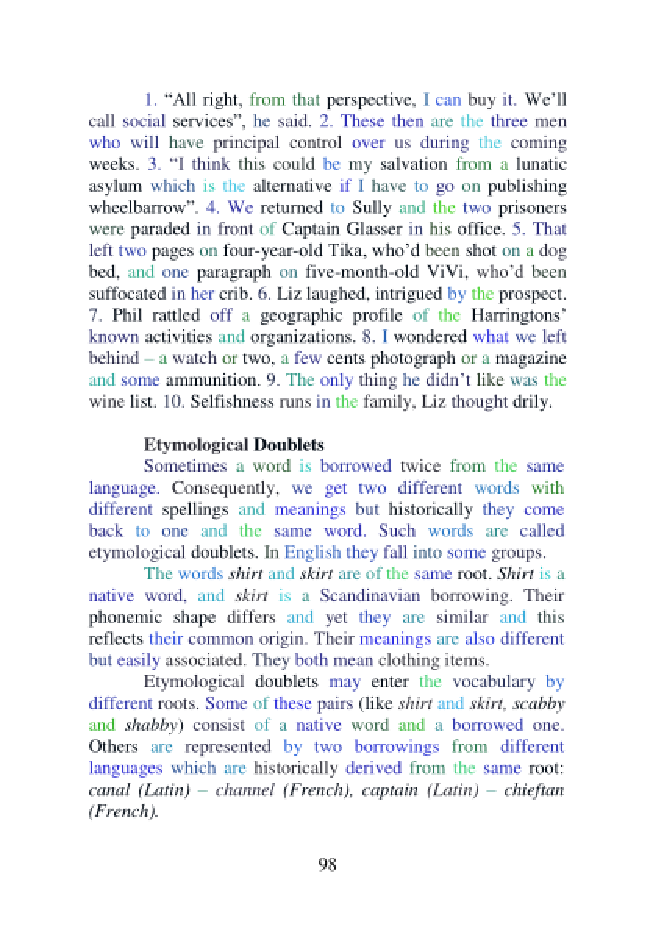
\includegraphics[width=\textwidth]{images/chapter4/plain.pdf}
        \caption{Plain}
      \end{subfigure}
      \begin{subfigure}[b]{0.24\textwidth}
        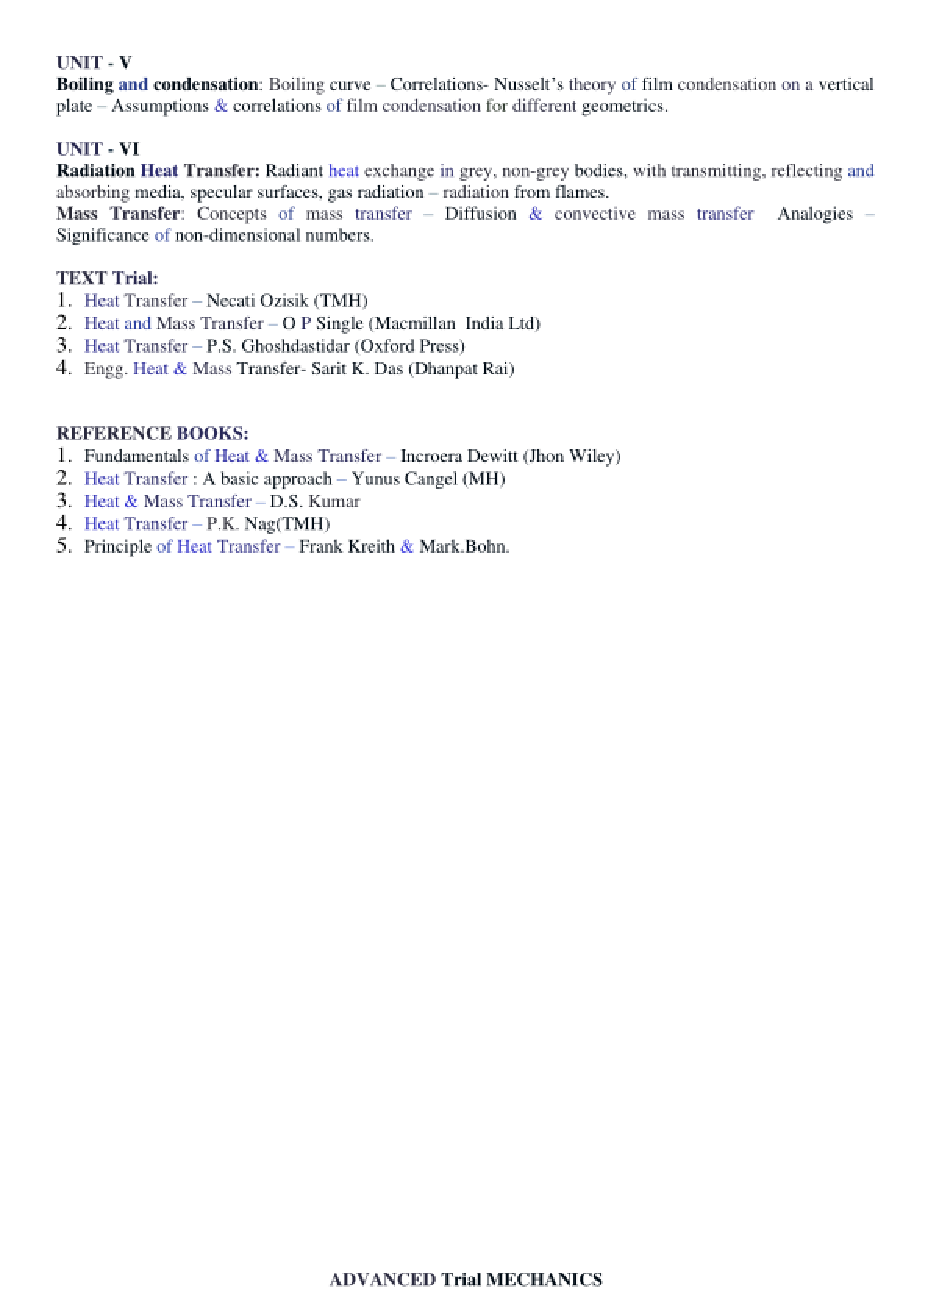
\includegraphics[width=\textwidth]{images/chapter4/list.pdf}
        \caption{List}
      \end{subfigure}
      \begin{subfigure}[b]{0.24\textwidth}
        
\includegraphics[width=\textwidth]{images/chapter4/multicolumn.pdf}
        \caption{Multicolumn}
      \end{subfigure}
      \begin{subfigure}[b]{0.24\textwidth}
        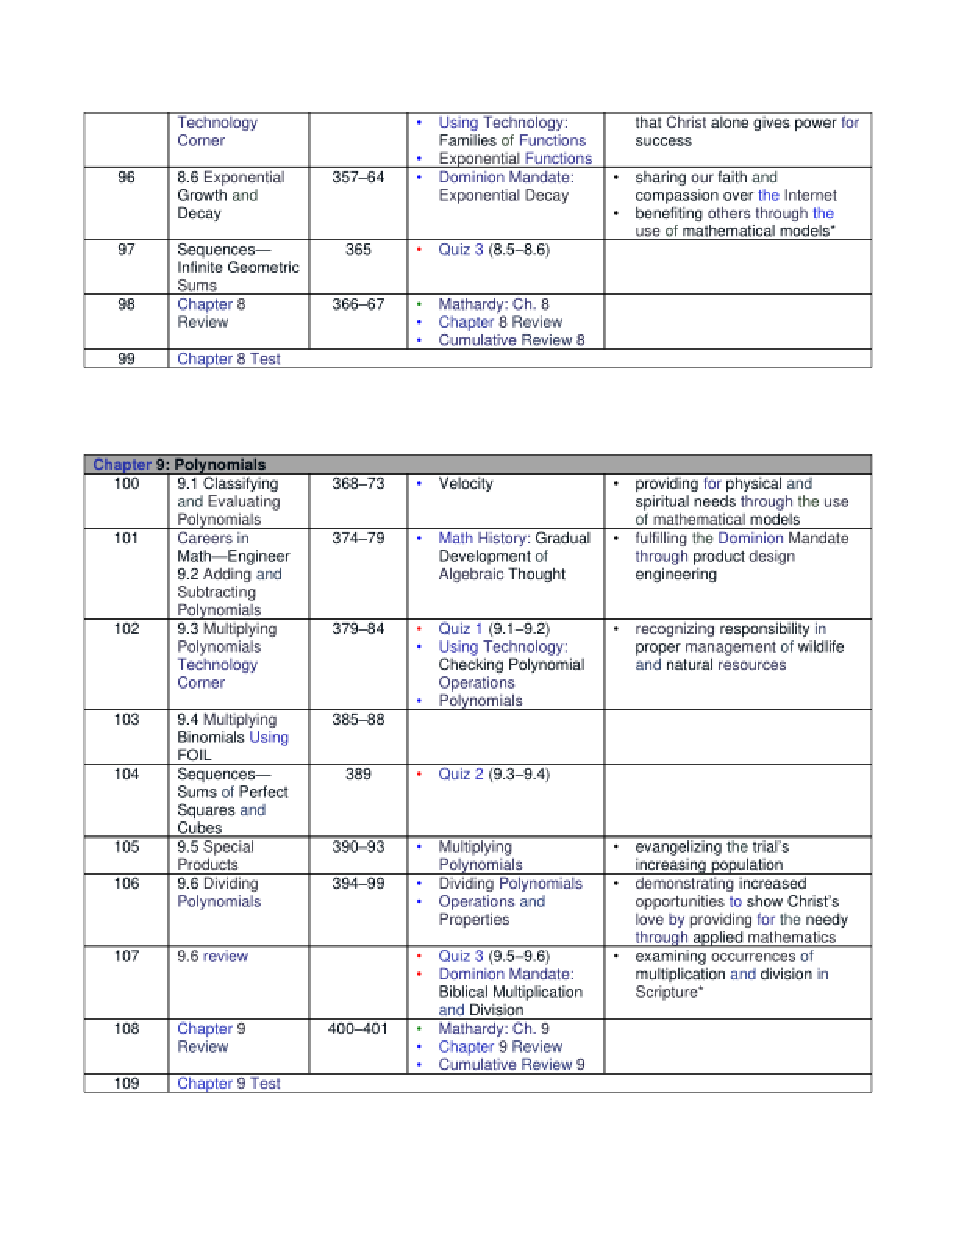
\includegraphics[width=\textwidth]{images/chapter4/tables.pdf}
        \caption{Table}
      \end{subfigure}
    \caption{Examples of documents for each layout category, arranged from the simplest to the most complex.}
    \label{fig:layout-examples}
\end{figure}

\begin{table}
  \centering
  \small
  \begin{adjustbox}{max width=\textwidth}
  \begin{threeparttable}
  \begin{tabular}{lcccccccc}
      \toprule
          & & \multicolumn{4}{c}{\textbf{Layout Type}} & \\
          & & \textbf{Plain} & \textbf{Lists} & \textbf{Multicolumn} & \textbf{Tables}\\
      \midrule
      Tesseract OCR \citep{kay2007tesseract} & & 78.71 & 72.75 & 61.43 & 36.97 \\
      DocTR \citep{doctr2021} & & 86.83 & 77.83 & 82.54 & 66.11 \\
  \bottomrule
  \end{tabular}
  \end{threeparttable}
  \end{adjustbox}
  \caption{Accuracy (in \%) obtained by each \ac{OCR} engine, for each document layout type.}
  \label{table:ocr-preliminary-experiments}
\end{table}

\begin{figure}
    \centering
    \small
      \begin{subfigure}[b]{\textwidth}
        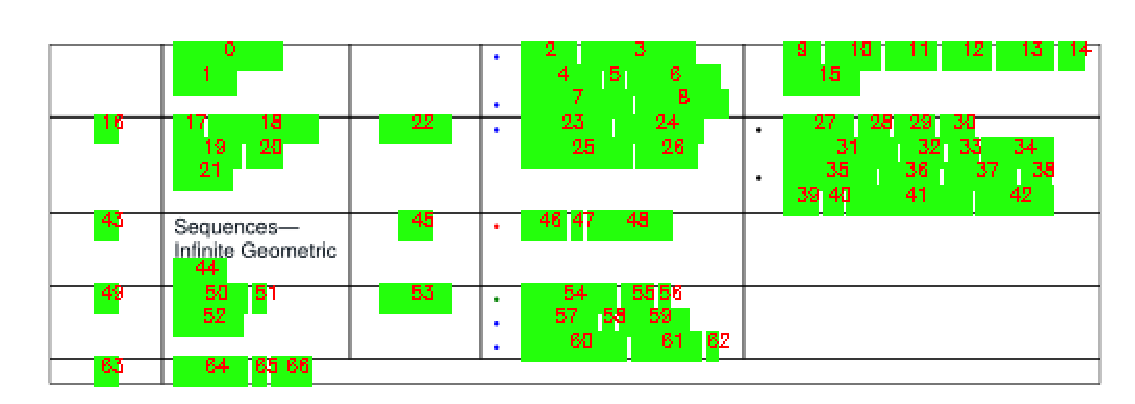
\includegraphics[width=\textwidth]{images/chapter4/gold_tables.pdf}
        \caption{Ground-truth reading order}
      \end{subfigure}
      \begin{subfigure}[b]{\textwidth}
        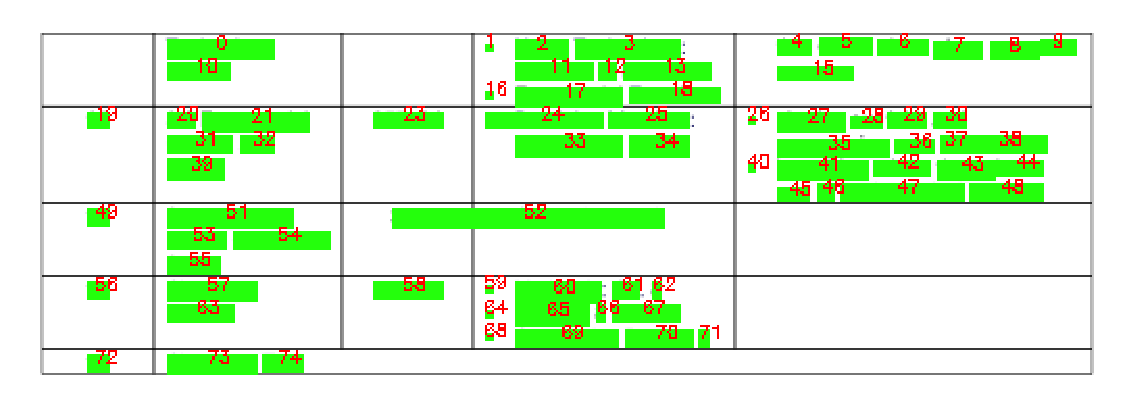
\includegraphics[width=\textwidth]{images/chapter4/tesseract_tables.pdf}
        \caption{Reading order obtained through Tesseract}
      \end{subfigure}
    \caption{Ground-truth reading order (a) compared to the reading order generated by Tesseract (b) for a sample table. Non-highlighted text indicates that it does not appear in the serialized sequence.}
    \label{fig:reading-orders-table}
\end{figure}

\begin{figure}
  \centering
  \small
      \begin{subfigure}[b]{0.5\textwidth}
        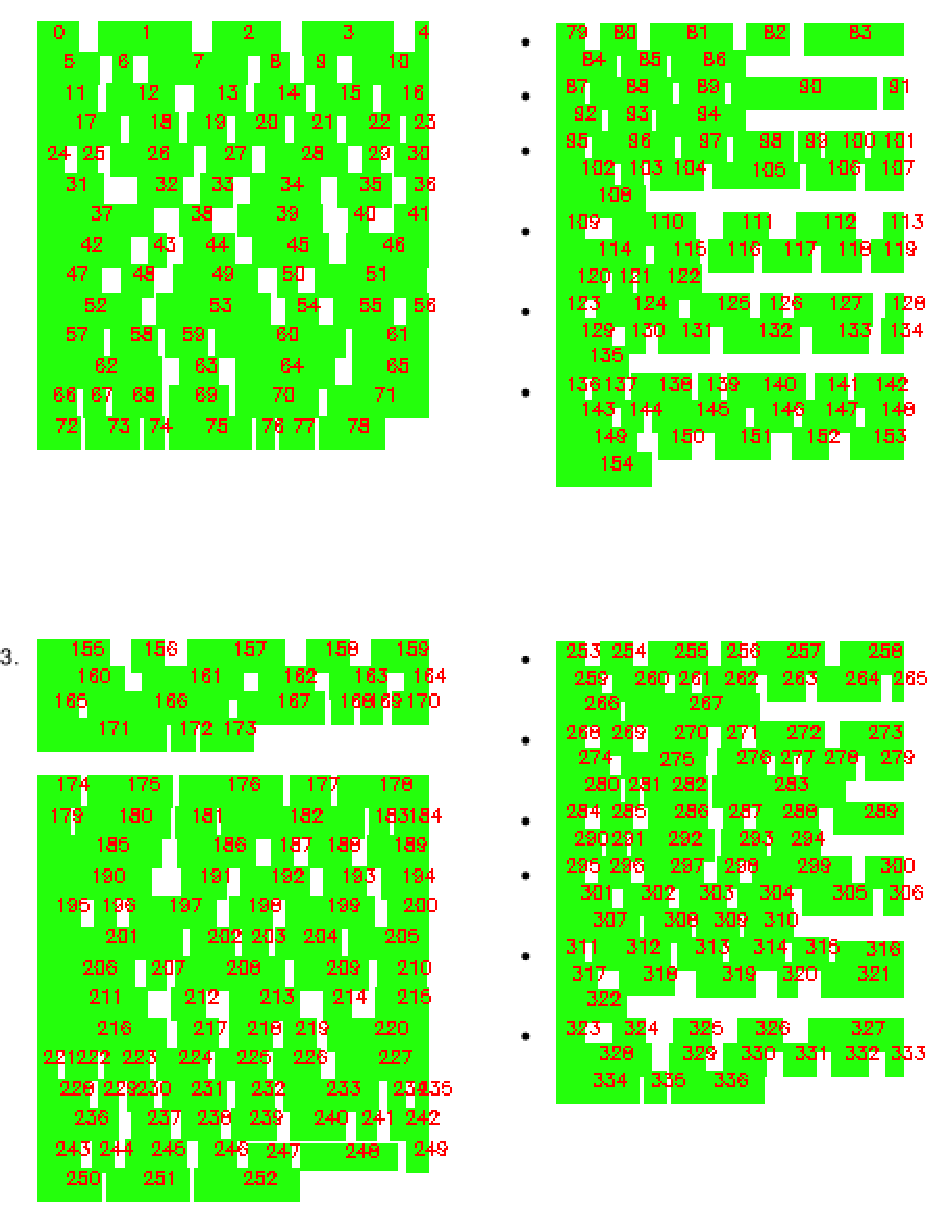
\includegraphics[width=\textwidth]{images/chapter4/gold_multicolumn.pdf}
        \caption{Ground-truth}
      \end{subfigure}
      \begin{subfigure}[b]{0.5\textwidth}
        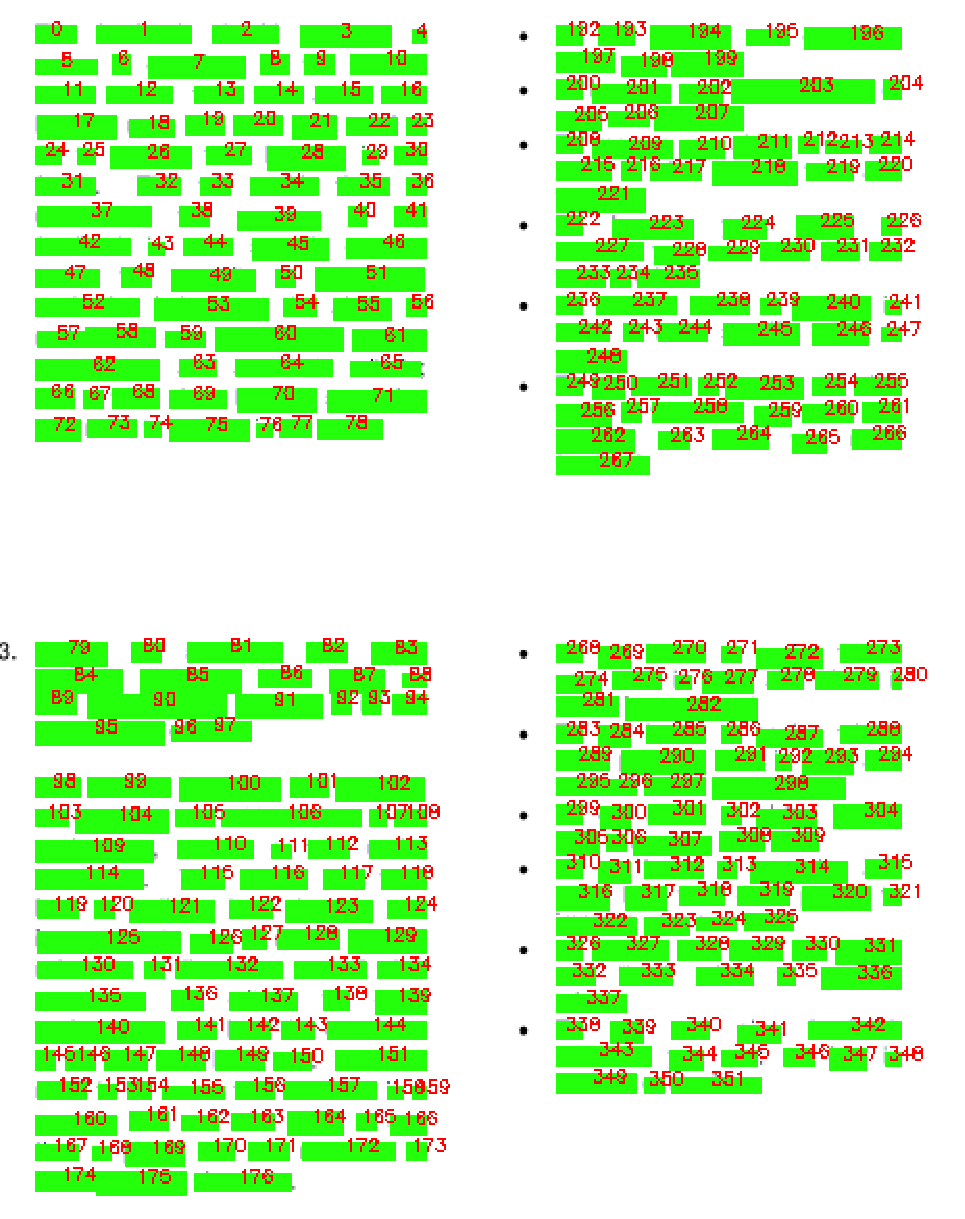
\includegraphics[width=\textwidth]{images/chapter4/tesseract_multicolumn.pdf}
        \caption{Tesseract}
      \end{subfigure}
    \caption{Ground-truth reading order (a) compared to the reading order generated by Tesseract (b) for a document with a two-column layout. The document was cropped for better visibility. Non-highlighted text indicates that it does not appear in the serialized sequence.}
    \label{fig:reading-orders-multicolumn}
\end{figure}


\subsection{Layout2Pos Module}

Building on the insights gained from the previous experiment, accurately retrieving the correct reading order poses a significant challenge for \ac{OCR} engines. We argue that it is possible to retrieve the correct reading order by leveraging the document layout. To address this, we propose a novel approach, \textit{Layout2Pos}, a transformer-based module that discards the reading order generated by \ac{OCR} and, instead, learns 1D position embeddings exclusively from the spatial positions of tokens. Layout2Pos is a stack of Transformer layers designed to generate a corresponding sequence of 1D position embeddings based on spatial information. In the following, we elaborate on the process of encoding spatial information into layout embeddings, followed by an in-depth description of our Layout2Pos module.

\subsubsection{Encoding Layout Information}

The spatial position of a token is represented by its bounding box in the document page image, denoted as $(x_0, y_0, x_1, y_1)$, where $(x_0, y_0)$ and $(x_1, y_1)$ correspond to the coordinates of the top-left and bottom-right corners, respectively. We discretize and normalize these coordinates to integers within the range of $[0, ..., 1000]$. Four embedding tables are employed to encode spatial positions: two for the coordinate axes ($x$ and $y$), and the other two for the bounding box size (width and height). In line with LayoutLMv2 \citep{xu2020layoutlmv2}, the final layout embedding $\bell \in \mathbb{R}^{d_{\ell}}$ of a token positioned at $(x_0, y_0, x_1, y_1)$ is defined as follows:

\begin{equation}
\begin{split}
    \bell & = \text{LayoutEmb}_x(x_0) \mathbin\Vert \text{LayoutEmb}_y(y_0) \\
    & \mathbin\Vert \text{LayoutEmb}_x(x_1) \mathbin\Vert \text{LayoutEmb}_y(y_1) \\
    & \mathbin\Vert \text{LayoutEmb}_w(x_1 - x_0) \mathbin\Vert \text{LayoutEmb}_h(y_1 - y_0), 
\end{split}
\label{eq:layout-embeddings}
\end{equation}

\noindent where $\mathbin\Vert$ denotes concatenation.

Following LayoutLMv2, we also encode spatial relative positions as bias terms added to the attention scores to explicitly capture the spatial relationship between tokens. For each pair of bounding boxes $((x_0, y_0, x_1, y_1), (x^{\prime}_0, y^{\prime}_0, x^{\prime}_1, y^{\prime}_1))$, we compute the horizontal distance $x^{\prime}_0 - x_0$ between the left edge of each box and the vertical distance $y^{\prime}_1 - y_1$ between the bottom edge of each box. To provide additional insights into the spatial relationships of tokens, we also compute the horizontal distance $x^{\prime}_1 - x_0$ between the right edge of one box and the left edge of the other (indicating information about the combined length). Furthermore, we calculate the horizontal distance $x^{\prime}_1 - x_1$ between the right edge of each box, providing information about the length of the second token in the pair. In addition, we consider \textit{line} and \textit{column} relative positions. Understanding the relative positions within lines helps the sequential structure of the document, aiding in distinguishing between different parts of the document. On the other hand, the relative positions within columns is valuable for documents with multicolumn layouts, offering insights into the spatial arrangement of text across columns. Overall, line and column information enhance the model's ability to capture the structural organization of textual content within documents. Hence, for each bounding box, we identify other bounding boxes that share the same line/column. This is determined by whether the horizontal/vertical line passing through the center of the box intersects with the other bounding boxes. If there is an intersection, the boxes are considered to be on the same line/column. For each token, we determine its positions within its corresponding line and column, employing a left-to-right order for lines and a top-to-bottom order for columns. Then, we compute the relative sequential distance $\delta^{line}_{ij}$ and $\delta^{column}_{ij}$ between elements within each line and column. If they do not belong to the same line or column, the distance is set to 1000. 

Formally, let $\bm{q}^{\ell}_i$ and $\bm{k}^{\ell}_i$ denote the query and key projections obtained from the layout embedding $\bell_i$ of token $i$. In Layout2Pos, attention is re-defined as:

\begin{equation}
  \begin{split}
  \alpha_{ij} &= \dfrac{1}{\sqrt{d}} \left(\bm{q}^{\ell}_i \cdot \bm{k}^{\ell}_j\right) \\
              & + b^{(2D_x)}_{x^{(j)}_{0} - x^{(i)}_{0}} + b^{(2D_y)}_{y^{(j)}_{1} - y^{(i)}_{1}} + b^{(2D_x)}_{x^{(j)}_{1} - x^{(i)}_{0}} + b^{(2D_x)}_{x^{(j)}_{1} - x^{(i)}_{1}} \\
              & + b^{(l)}_{\delta^{l}_{ij}}  + b^{(c)}_{\delta^{c}_{ij}},
  \end{split}
  \label{eq:layout2pos-attention}
\end{equation}

\noindent where $\bm{b}^{(2D_x)}$, $\bm{b}^{(2D_y)}$, $\bm{b}^{(l)}$, and $\bm{b}^{(c)}$ correspond to the horizontal, vertical, line, and column relative position biases, respectively. The biases are different among attention heads but shared across all layers. The relative sequential distances between elements within lines and columns, $\bm{\delta}^{(line)}$ and $\bm{\delta}^{(column)}$, are defined as follows:

\begin{equation}
  \begin{split}
    \delta^{l}_{ij} &= 
        \begin{cases}
          posInLine(j) - posInLine(i), & \text{if } line(j) = line(i)\\
            1000,              & \text{otherwise}.
        \end{cases} \\
    \delta^{c}_{ij} &= 
      \begin{cases}
        posInColumn(j) - posInColumn(i), & \text{if } column(j) = column(i)\\
          1000,              & \text{otherwise}.
      \end{cases}
  \end{split}
\end{equation}

\subsubsection{Learning 1D Position Embeddings from Layout Information}

\begin{figure}
  \centering
  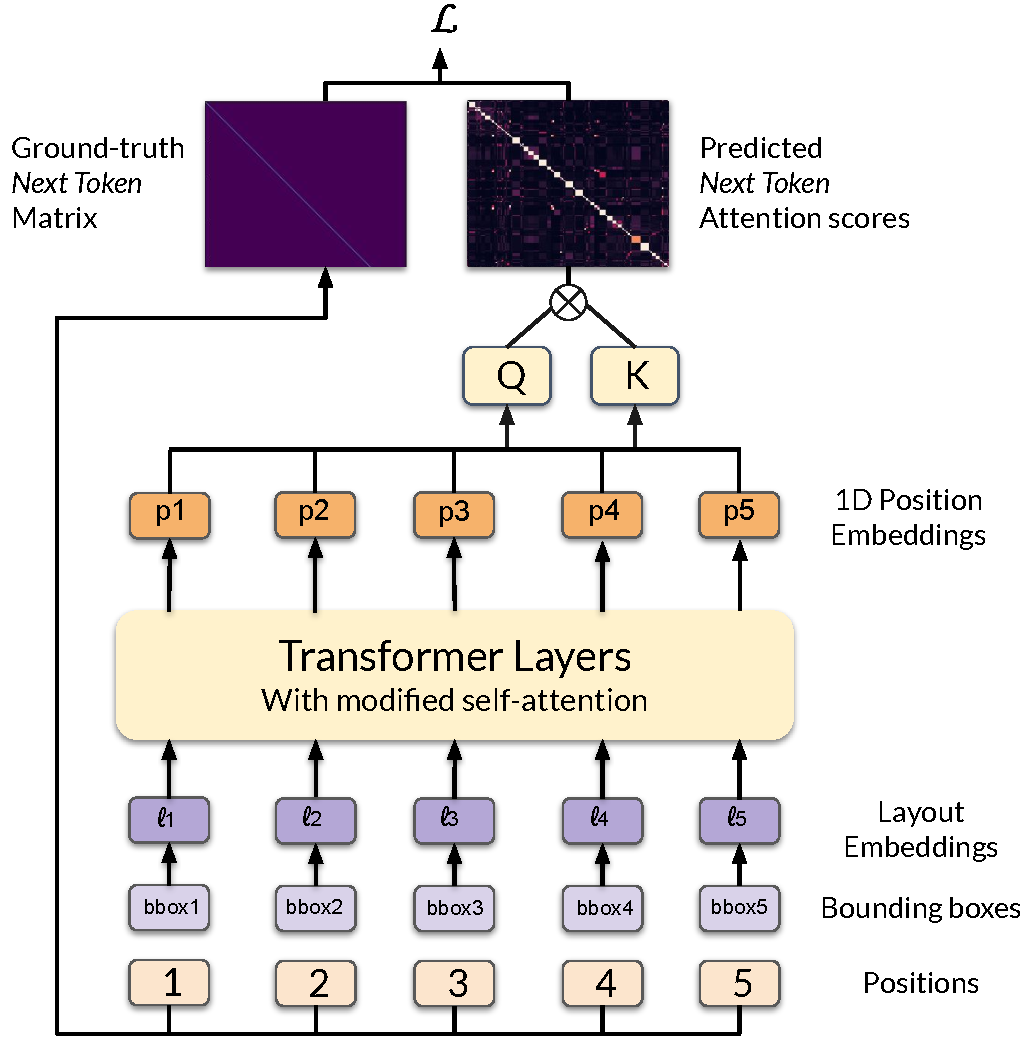
\includegraphics[width=0.75\textwidth]{images/chapter4/Layout2Pos.pdf}
  \caption{Layout2Pos Architecture. The input consists of a sequence of token bounding box coordinates, transformed into corresponding embedding sequences. Self-attention in the stack of Transformer layers is modified as defined by Equation~\ref{eq:layout2pos-attention}. $\bm{Q}$ and $\bm{K}$ are the queries and keys obtained by projecting the 1D position embeddings. The attention scores obtained through dot-product are compared against the ground-truth matrix to compute the Next Token Position Prediction loss.}
  \label{fig:layout2pos-module}
\end{figure}

Given a sequence of layout embeddings as defined by Equation~\ref{eq:layout-embeddings}, Layout2Pos employs a stack of $M$ Transformer layers to contextualize the sequence. The outputs of the last layer serve as 1D position embeddings:

\begin{equation}
  \bm{p}_i = \bm{h}^M(\bell_i).
\end{equation}

\noindent Then, these 1D position embeddings are used to compute the attention matrix $\bm{A}$, \textit{i.e.}, alignment scores between every token:

\begin{equation}
  A_{ij} = \left(\bm{p}_i \bm{W}^q\right)\left(\bm{p}_j \bm{W}^k\right).
\end{equation}

\noindent We assume that the attention matrix $\bm{A}$ carries information about the reading order, \textit{i.e.}, $A_{ij}$ represents the probability that the $j$-th token follows the $i$-th token. Let $N$ denote the ground-truth binary matrix obtained from the ground-truth reading order, where $N_{ij}$ equals $1$ if token at position $j$ is the \textit{next} token after token at position $i$ in the sequence, and $0$ otherwise. We define the \textit{Next Token Position Prediction} strategy, which consists in using the attention matrix $\bm{A}$ to predict the next token of each token in the sequence (\textit{next token matrix}). The corresponding loss is defined as follows:

\begin{equation}
  \mathcal{L}_{NTP} = - \sum_{i=1}^n \sum_{j=1}^n N_{ij} \log\left(\textrm{softmax}(A_{ij})\right).
\end{equation}

\noindent As such, Layout2Pos is trained to capture the relationship between spatial arrangement of tokens and reading order. This is done by ensuring that the attention matrix $\bm{A}$ derived from the computed 1D position embeddings carries information about the next token for each token in the sequence. The architecture of Layout2Pos is depicted in Figure~\ref{fig:layout2pos-module}. It is noteworthy that a global reading order is unnecessary; there is no requirement to establish an order between two words that belong to segments that have no relation to each other.

% Given that each token is treated as a bounding box defined by its size and position, a significantly smaller representation space can be chosen for layout features compared to text. As Layout2Pos does not need to understand semantic content, it may require a smaller latent space dimension than conventional multimodal pre-trained models. 

\subsubsection{Integrating Layout2Pos into a Sequence-to-Sequence Framework}

\begin{figure}
  \centering
  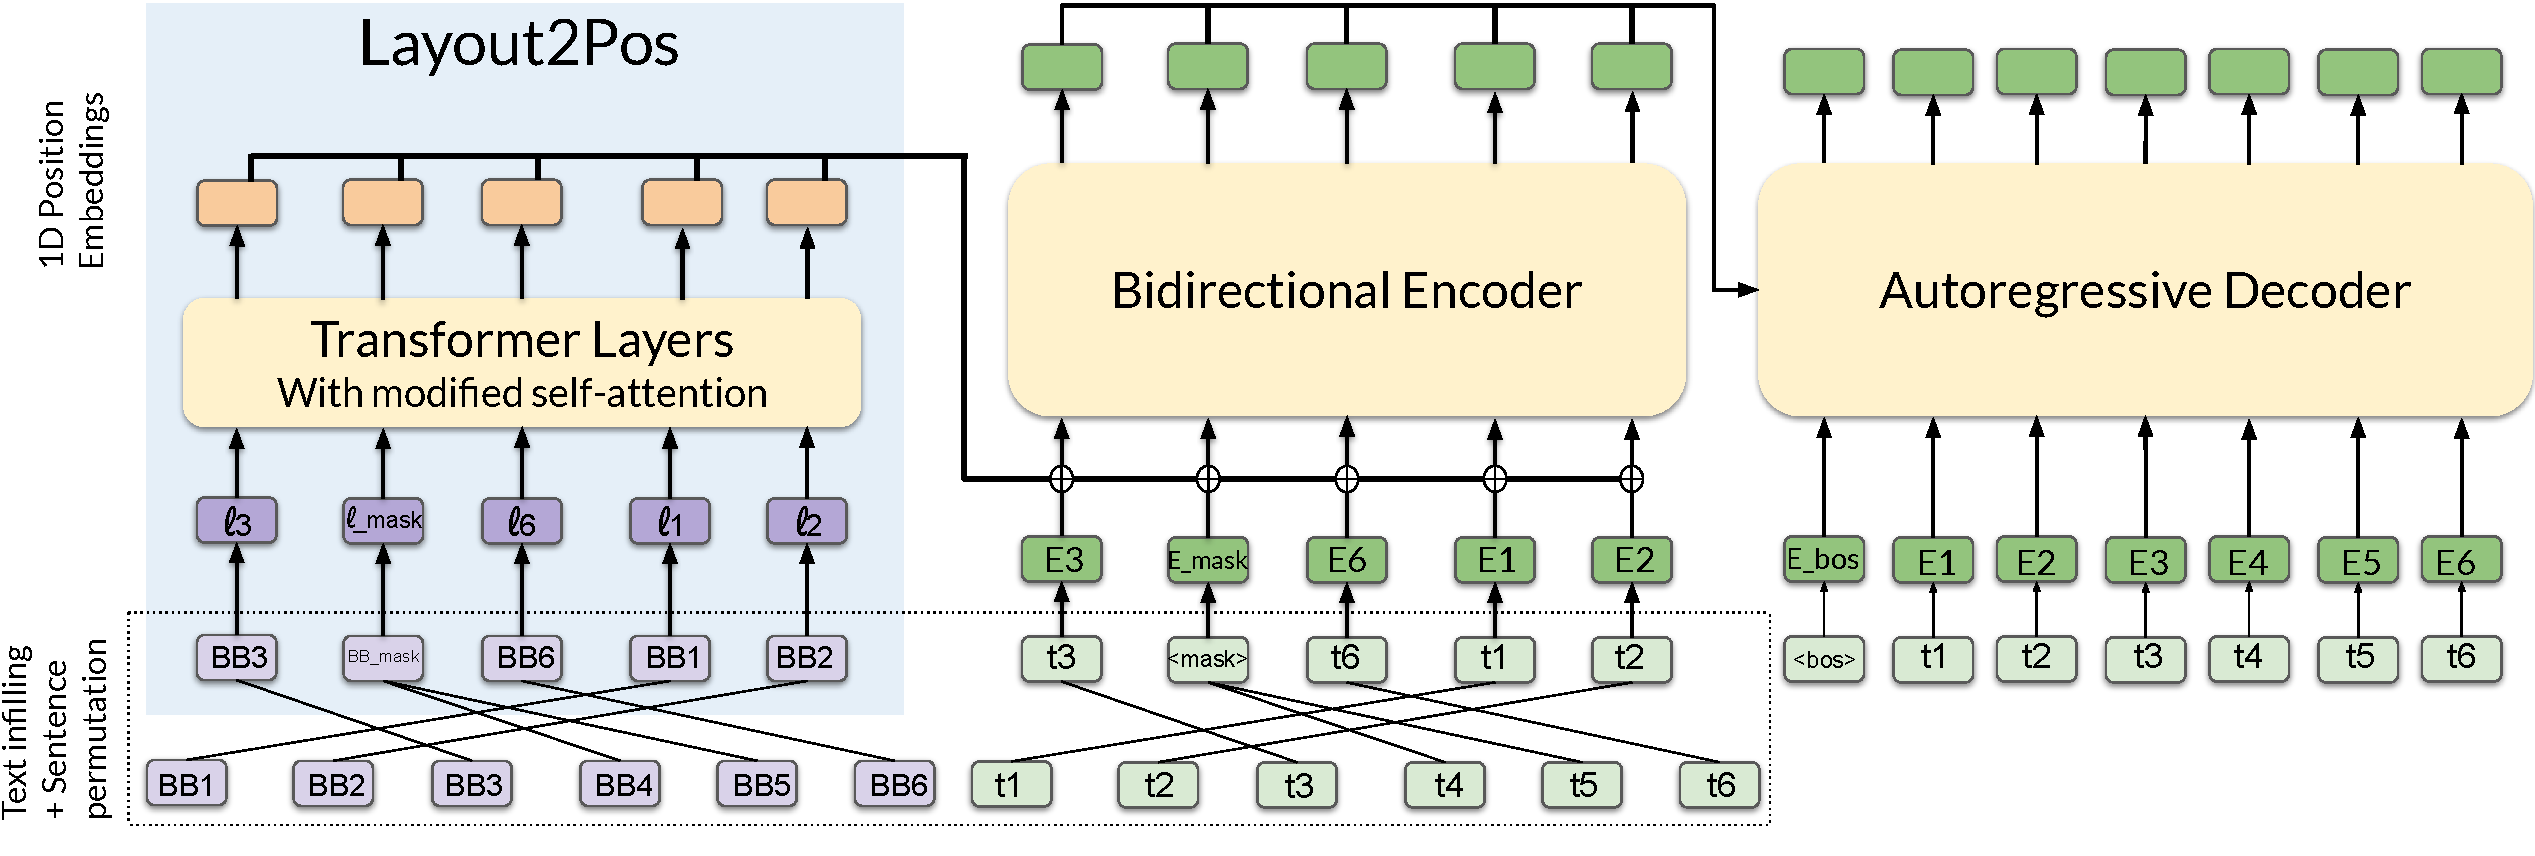
\includegraphics[width=\textwidth]{images/chapter4/Layout2Pos+BART.pdf}
  \caption{Architecture of Layout2Pos integrated into a BART model, \textit{i.e.}, BART+Layout2Pos. The input consists of two components: a sequence of tokens and a sequence of token bounding box coordinates. The sequence of tokens is corrupted using \textit{text infilling and sentence permutation}, and the sequence of token bounding boxes is altered accordingly. Both  sequences are transformed into corresponding embedding sequences. Layout2Pos learns to calculate 1D position embeddings from layout embeddings using the \textit{next token position prediction} loss. The sequence of 1D position embeddings are subsequently added to the token embeddings. The resulting embeddings are fed into an encoder-decoder model, trained to reconstruct the original sequence of tokens (\textit{denoising}).}
  \label{fig:layout2pos-ed}
\end{figure}

Layout2Pos can be integrated into any language model, removing the reliance on sequential position information. This is achieved by substituting the traditional 1D position encodings derived from \ac{OCR} by the 1D position embeddings produced by Layout2Pos. Specifically, we integrate Layout2Pos into a Transformer encoder-decoder architecture, as illustrated in Figure~\ref{fig:layout2pos-ed}. The model receives a sequence of tokens and the corresponding sequence of token bounding boxes as input, both embedded using embedding tables. The sequence of position embeddings, obtained by Layout2Pos, is added to the sequence of token embeddings, and the resulting sequence is input to the bidirectional encoder. The output sequence of contextualized embeddings is fed to the autoregressive decoder to generate the target sequence.

\paragraph{Training} Layout2Pos is simultaneously trained with the encoder-decoder model. While the module learns to predict the subsequent token of each token based on layout information, the encoder-decoder follows a pre-training approach similar to \ac{BART}  \citep{lewis2006building}. The model is trained to reconstruct the original input sequence from a corrupted version (\textit{denoising}). Sequences are corrupted by randomly replacing text spans with a single mask token (\textit{text infilling}) and permuting sentences (\textit{sequence permutation}). The corrupted sequence is encoded using the bidirectional encoder, and the autoregressive decoder is trained to reconstruct the original sequence. We refer to the overall model as BART+Layout2Pos.

\paragraph{Inference} To determine how the model predicts the next token of the sequence, BART+Layout2Pos employs a customized variant of beam search to generate tokens while minimizing repetitions. In this modified version, the generated tokens, if already present in the source sequence, are constrained not to occur more frequently than in the original source. This constraint is enforced by keeping count of the number of occurrences of each token in the source sequence within the target sequence and masking the corresponding logit when the maximum occurrence is reached. This approach aims to enhance the coherence of the generated sequences by ensuring that the generated tokens align appropriately with the content of the input document, minimizing redundancy and improving overall output quality.


\section{Experiments and Results}

In this section, we provide an overview of the datasets used for pre-training our models and conducting visual information extraction tasks. Furthermore, we provide details on the experimental setup, covering baselines, pre-training methodologies, and fine-tuning protocols. We evaluate our models on the Next Token Position Prediction task, along with three benchmark visual information extraction tasks. 

\subsection{Data}

\subsubsection{Pre-training Data}

Following a common practice in the field of Document Understanding, we collect data from the IIT-CDIP collection \citep{lewis2006building} to build our pre-training dataset. IIT-CDIP consists of around 11 million document page images of various types and layouts, including news articles, scientific reports, handwritten materials, and more. The collection contains scanned images of documents, introducing challenges related to image quality, resolution, and potential artifacts. As such, we leverage IIT-CDIP to pre-train models under realistic conditions. We select over 7 million document images from the collection to build our pre-training dataset. To extract text and bounding boxes from the documents, we use DocTR \citep{doctr2021}. Due to potential serialization errors induced by DocTR, and given that the Next Token Position Prediction task requires documents with proper reading orders, IIT-CDIP is only used for training models in language modeling tasks (\textit{i.e.}, text infilling and sequence permutation). 

To enable Layout2Pos to effectively learn the correct reading order of documents, we use the 500k documents from the ReadingBank dataset \citep{wang2021layoutreader}. These documents are serialized and annotated with high-quality reading order annotations, serving as the training data for both Next Token Position Prediction and language modeling tasks. 

Our final pre-training corpus is referred to as IIT-CDIP+ReadingBank. While permutation is used for both datasets, text infilling is not applied to ReadingBank. This choice is made to prevent potential alignment issues between next token position prediction and language modeling, which could arise from replacing spans of tokens with a single mask token.

In cases where a word is split into multiple tokens, earlier approaches based on word-level bounding boxes typically assign the word's bounding box to all the tokens within that word. However, this approach is inefficient for next token position prediction, given that tokens within the same word would share identical layout embeddings, hence hindering accurate predictions of the next token. Therefore, we approximate token-level bounding boxes by dividing each word-level bounding box by the number of characters in the word.

\subsubsection{Data for Visual Information Extraction}

We evaluate our approach on visual information extraction tasks, where the goal is to extract semantic entities from visually-rich documents, based on a set of pre-defined keys. This evaluation is conducted using three benchmark for visual information extraction, each covering different document types: FUNSD \citep{jaume2019funsd}, CORD \citep{park2019cord}, and SROIE \citep{huang2019icdar2019}. For each dataset, we use the reading order provided. To maintain consistency with pre-training data, we employ approximated token-level bounding boxes.

\paragraph{FUNSD} \citep{jaume2019funsd} is a form understanding dataset consisting of 199 real, noisy and scanned forms where each sample contains a list of form entities. There are three keys for which values have to be extracted: \textit{question}, \textit{answer}, and \textit{header}. The dataset is split into 149 samples for training and 50 for test.

\paragraph{CORD (v1)} \citep{park2019cord} is a receipt understanding dataset containing 1,000 scanned Indonesian receipts with 30 keys categorized into four superclasses: \textit{menu}, \textit{subtotal}, \textit{total}, and \textit{void}. We exclude keys with very few occurrences,\footnote{Discarded keys are: menu.etc, menu.itemsubtotal, menu.sub\_etc, menu.sub\_unitprice, menu.vatyn, void\_menu.nm, void\_menu.price, sub\_total.othersvc\_price.} which results in 22 keys grouped into three superclasses. The dataset is divided into 800 examples for training, 100 for validation, and 100 for test.

\paragraph{SROIE} \citep{huang2019icdar2019} is another receipt understanding dataset comprising 973 scanned receipts written in English. The task involves extracting entities for four keys: \textit{total}, \textit{date}, \textit{company}, and \textit{address}. The dataset is partitioned into 626 samples for training and 347 for test. 

\subsection{Experimental Settings}

Models were implemented in Python using PyTorch \citep{paszke2017automatic} and Hugging Face \citep{wolf2019huggingface} librairies. 

\subsubsection{Baselines}

We compare our approach with BART+2D, a layout-augmented \ac{BART} model which relies on 1D position embeddings derived from \ac{OCR}-induced positions. These 1D position embeddings are calculated using embedding tables and are subsequently added to textual features. Layout embeddings, computed from bounding boxes using Equation~\ref{eq:layout-embeddings}, are incorporated to the resulting embeddings to construct the input embeddings. Following LayoutLMv2 \citep{xu2020layoutlmv2}, self-attention is modified as follows: 

\begin{equation}
  \alpha_{i,j} = \dfrac{1}{\sqrt{d}} \bm{q}_i \cdot \bm{k}_j + b^{(1D)}_{j - i} + b^{(2D_x)}_{x^{(j)}_{0} - x^{(i)}_{0}} + b^{(2D_y)}_{y^{(j)}_{1} - y^{(i)}_{1}},
\end{equation}

\noindent where $\bm{b}^{(1D)}$, $\bm{b}^{(2D_x)}$, and $\bm{b}^{(2D_y)}$ denote the sequential, horizontal, and vertical relative position biases, respectively. BART+2D follows the same training and inference procedures as BART+Layout2Pos.

Additionally, we report the performance of two layout-aware encoder-only models. We use LayoutLM and a variant of LayoutLMv2 that discards visual information (referred to as LayoutLMv2-no-visual), ensuring a fair comparison with our approach. 

\subsubsection{Pre-training}

\paragraph{Encoder-decoder Models} Layout2Pos is composed of 2 layers with 12 attention heads and a hidden size of 768. The final attention calculation, responsible for computing the next token matrix, involves a single attention head. Following the \ac{BART} base model, both the encoder and decoder in BART+Layout2Pos and BART+2D are comprised of 6 layers, each with 12 attention heads and a representation space dimensionality of 768. BART+Layout2Pos encompasses a total of 156 million parameters, while BART+2D amounts to 140k parameters. 

Both models are trained from scratch on IIT-CDIP+ReadingBank. The documents are tokenized 
using the tokenizer of the base variant of \ac{BART} (bart-base) shared through the Hugging Face Model Hub. The training spans 10 epochs, amounting to 500k optimization steps, including 59k for warmup. For each model, we select the checkpoint with the best validation loss. We use a maximum sequence length of 512, a batch size of 80, and a learning rate of 1e-4. For text infilling, we set the masking ratio to 0.3, with span lengths drawn from a Poisson distribution where $\lambda$ equals 3. Every sentence is permuted. Experiments were ran on Nvidia Titan RTX with 25GB. 

\paragraph{Encoder-only baselines} For LayoutLM, the microsoft/layoutlm-base-uncased checkpoint with 113M parameters is used. Following the base architecture of LayoutLMv2, LayoutLMv2-no-visual is composed of a 12-layer Transformer encoder with 12 attention heads and a hidden size of 768, amounting to 110M parameters. The model is also pre-trained from scratch, using \ac{MVLM} on IIT-CDIP+ReadingBank. The documents are tokenized using the tokenizer of microsoft/layoutlm-base-uncased. The pre-training extends over 10 epochs, with a maximum sequence length of 512, a batch size of 80, and a learning rate of 1e-4.


\subsubsection{Visual Information Extraction}

\paragraph{Sequence-labeling approaches}

To compare our sequence-to-sequence approach with the traditional sequence labeling method on visual information extraction tasks, we employ LayoutLM and LayoutLMv2-no-visual. For every dataset, the maximum sequence length is set to 512. Both models are fine-tuned for 100 on FUNSD, and 20 epochs on SROIE and CORD. The learning rate is set to 5e-5 for all models and datasets.

\paragraph{Sequence-to-sequence models} We frame visual information extraction as a sequence-to-sequence problem, wherein the document serves as the input, and the output consists of a series of extracted entities paired with their corresponding keys. In Figure~\ref{fig:source-target-sample}, we provide an example of a source document from SROIE and its corresponding target sequence. 

Entities and their corresponding keys are extracted from both the generated sequences and the ground-truth sequences. The pairs of generated and ground-truth \textit{(key, entities)} are then compared to compute precision, recall, and F1 score. To provide further insights into the model's errors, additional metrics are defined. The \textit{hallucination rate} represents the percentage of entities generated by the model that do not match with any text in the input sequence. It is used to measure how often the model produces content that is not grounded in the input. The \textit{repetition rate} is the percentage of entities that are part of the ground-truth entities but are repeated excessively. It quantifies the frequency with which the model generates duplicated entities. The \textit{wrong label rate} represents the proportion of generated entities present in the ground-truth but mislabeled by the model. It measures how often the model generates the right entities but mislabels them. The \textit{omission rate} denotes the proportion of ground-truth entities that were not generated by the model, providing insights into how often the model omits entities. Lastly, the \textit{non-entity rate} is the percentage of generated entities that, in the ground-truth, correspond to the category "Other". This metric assesses the frequency with which the model categorizes a text as an entity when it is not.

% We attribute the improvement to the fact that, although the advanced serialization is not used for fine-tuning datasets, the model has the ability to understand the proper reading order of documents after pre-training.

For all three datasets, we set the maximum source sequence length to 512. Documents that exceed this length are split into sequences, each consisting of 512 tokens. For each input sequence, we formulate a target sequence containing the pairs of values-keys contained in the input sequence. In the case of FUNSD, we truncate target sequences at 768 tokens. As for SROIE and CORD, the maximum target sequence length is set to 96 and 512 tokens, respectively. Models are fine-tuned for 30 epochs on CORD. The learning rate is set to 5e-5 for all models and datasets. During inference, we set the number of beams to 8.

% Models are fine-tuned for 100 epochs on FUNSD and 10 on CORD. As for SROIE, fine-tuning is conducted for 40 epochs for BART+2D and 100 epochs for BART+Layout2Pos. The learning rate is set to 5e-5 for all models and datasets. During inference, we set the number of beams to 5.

Considering that the pre-training phase has allowed BART+Layout2Pos to understand the correct reading order of documents, and acknowledging the potential discrepancies in the reading order within visual information extraction datasets, we opt not to use the Next Token Position Prediction strategy during fine-tuning.

% \begin{figure}
%   \centering
%   \small
%       \begin{subfigure}[b]{0.3\textwidth}
%         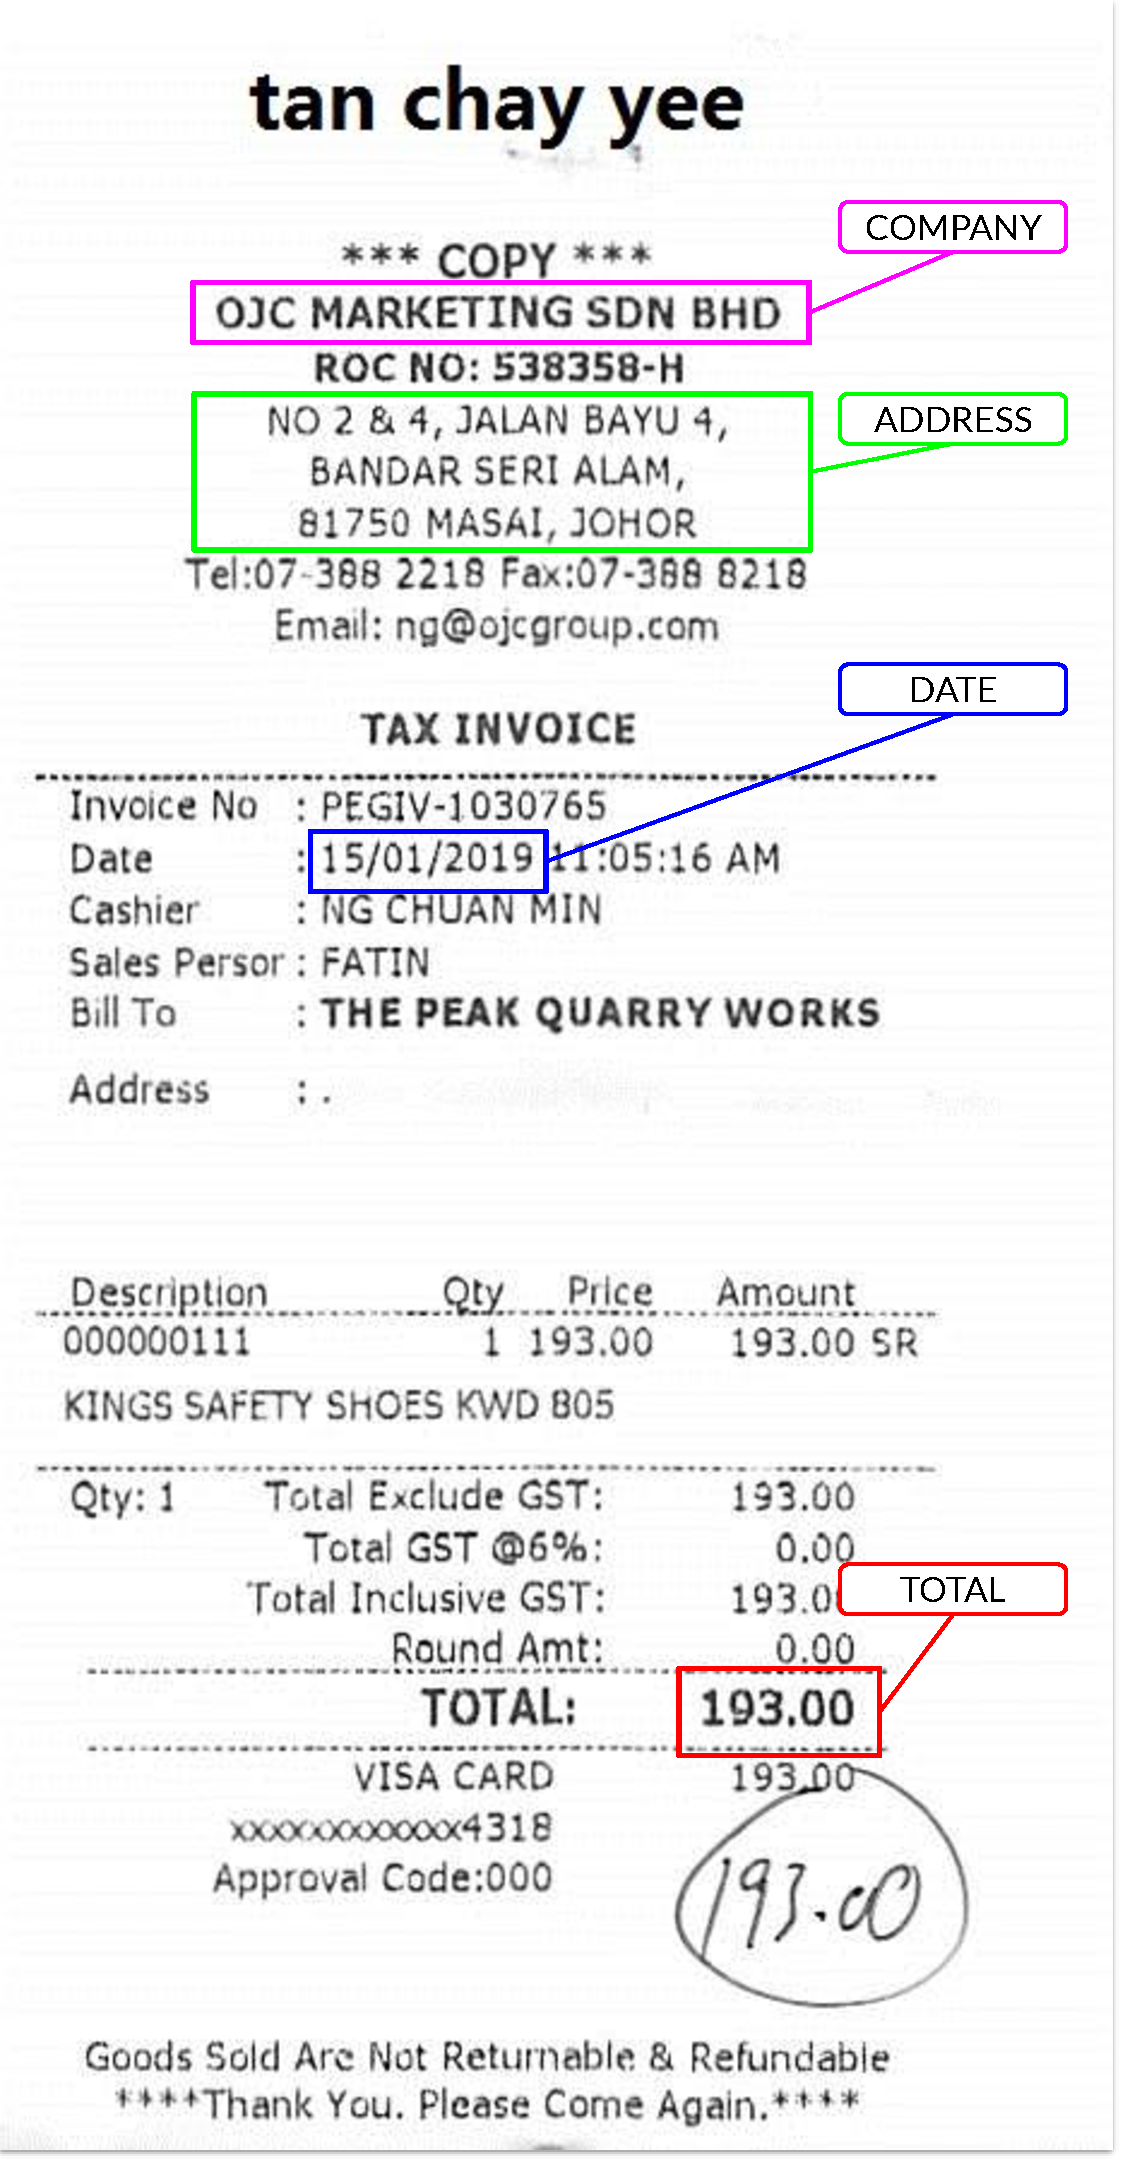
\includegraphics[width=\textwidth]{images/chapter4/sroie_sample.pdf}
%         \caption{Source document}
%       \end{subfigure}
%       \begin{subfigure}[b]{0.25\textwidth}
%         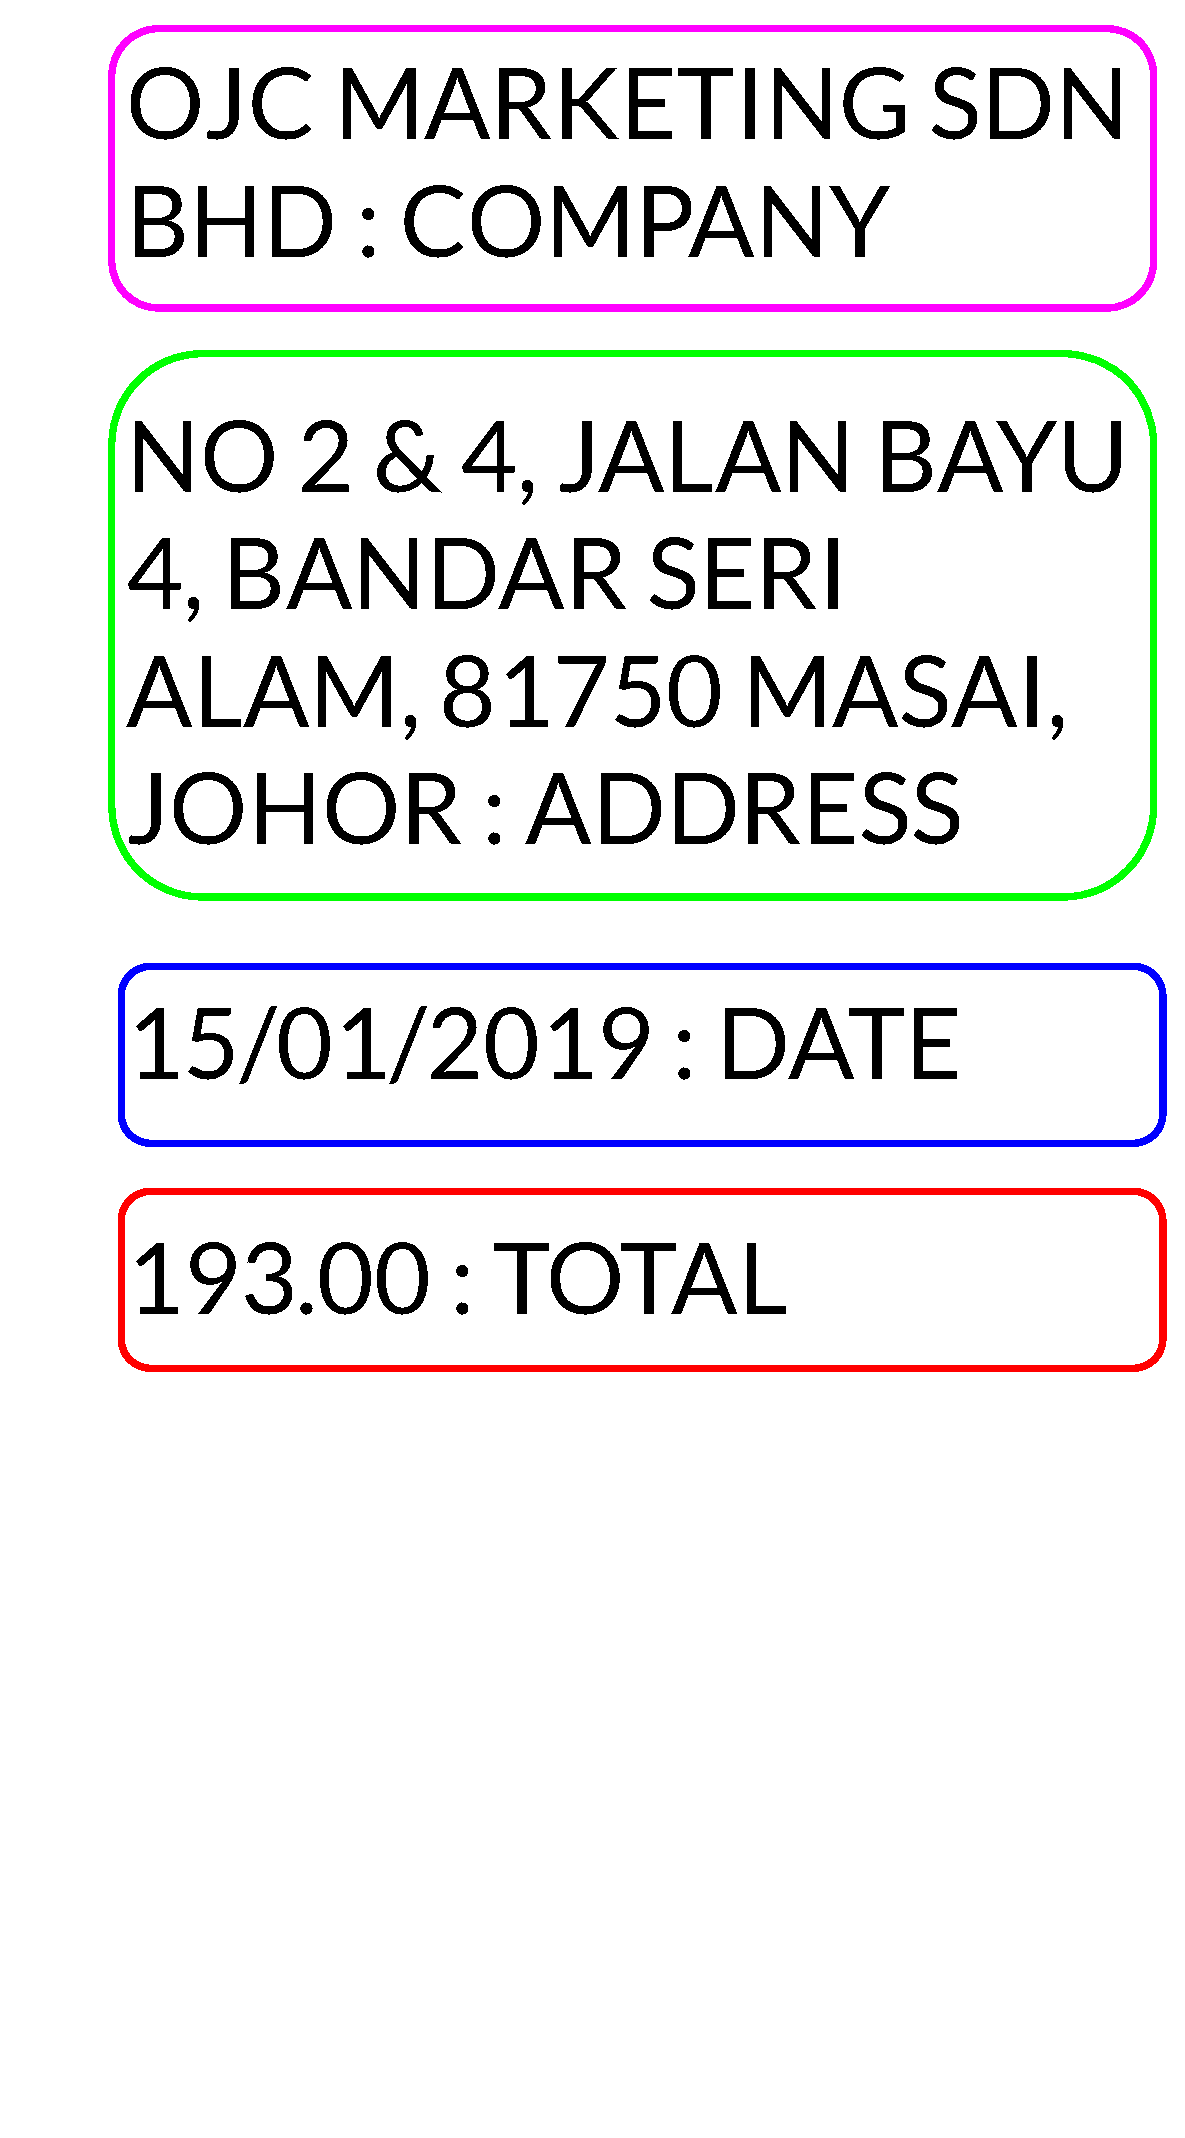
\includegraphics[width=\textwidth]{images/chapter4/sroie_output_sample2.pdf}
%         \caption{Target text}
%       \end{subfigure}
%     \caption{Example document from SROIE, accompanied by its corresponding target sequence that includes the entities to be extracted paired with their corresponding keys.}
%     \label{fig:source-target-sample}
% \end{figure}

\begin{figure}
  \centering
  \small
  \begin{subfigure}[b]{0.6\textwidth}
    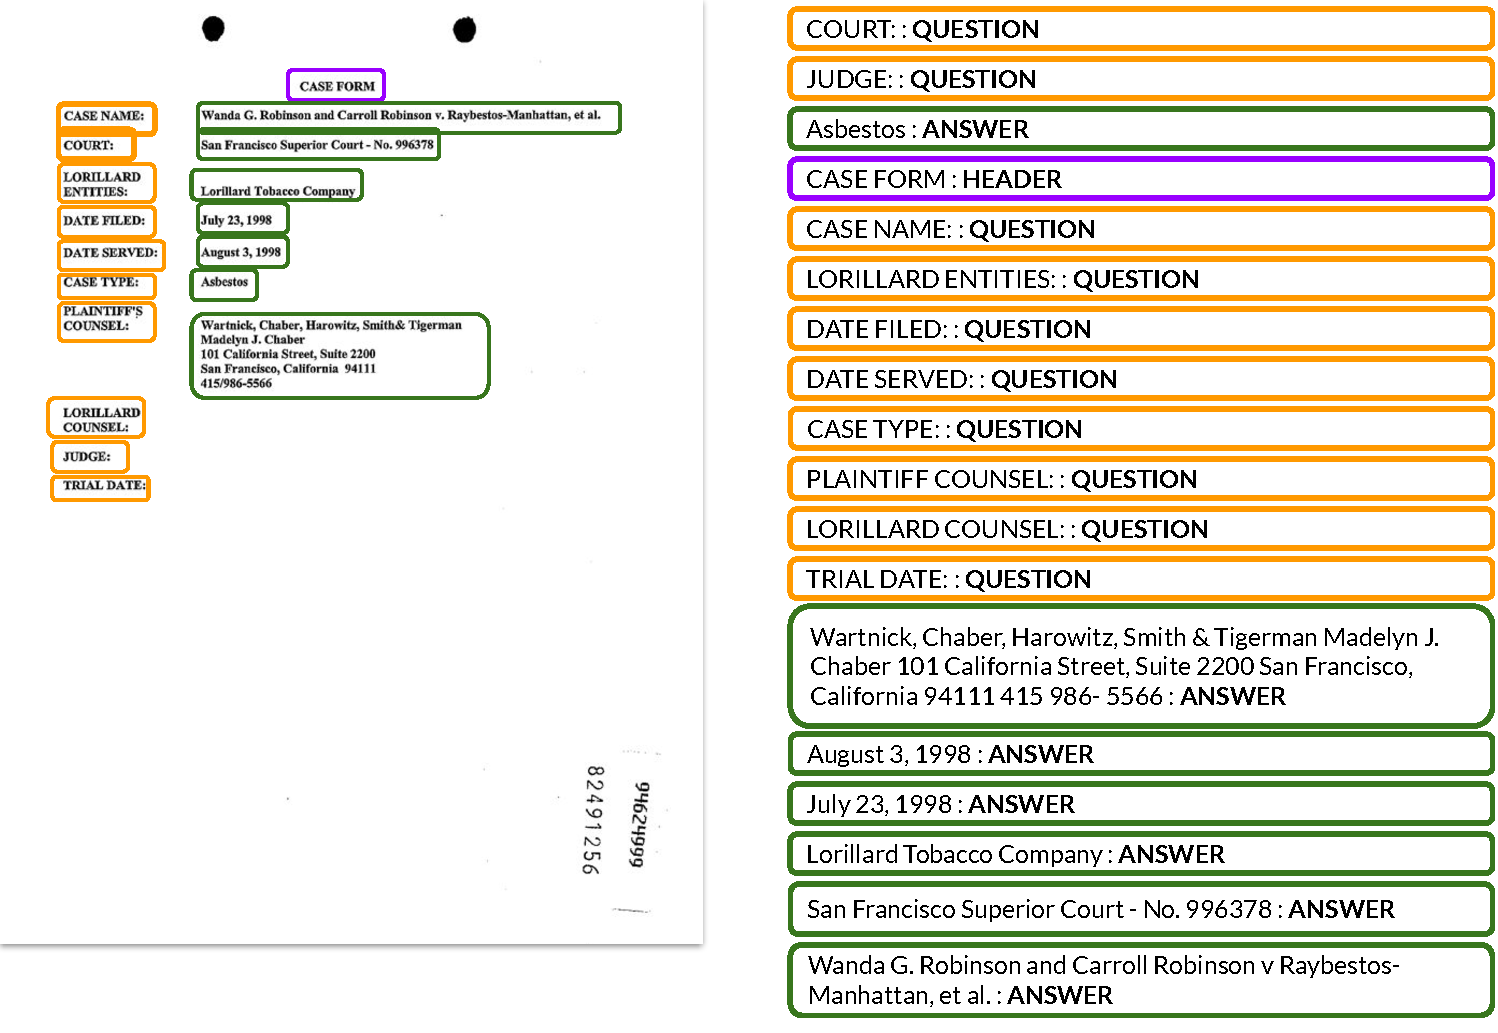
\includegraphics[width=\textwidth]{images/chapter4/funsd_sample_and_output.pdf}
    \caption{FUNSD}
  \end{subfigure}
  \begin{subfigure}[b]{0.4\textwidth}
    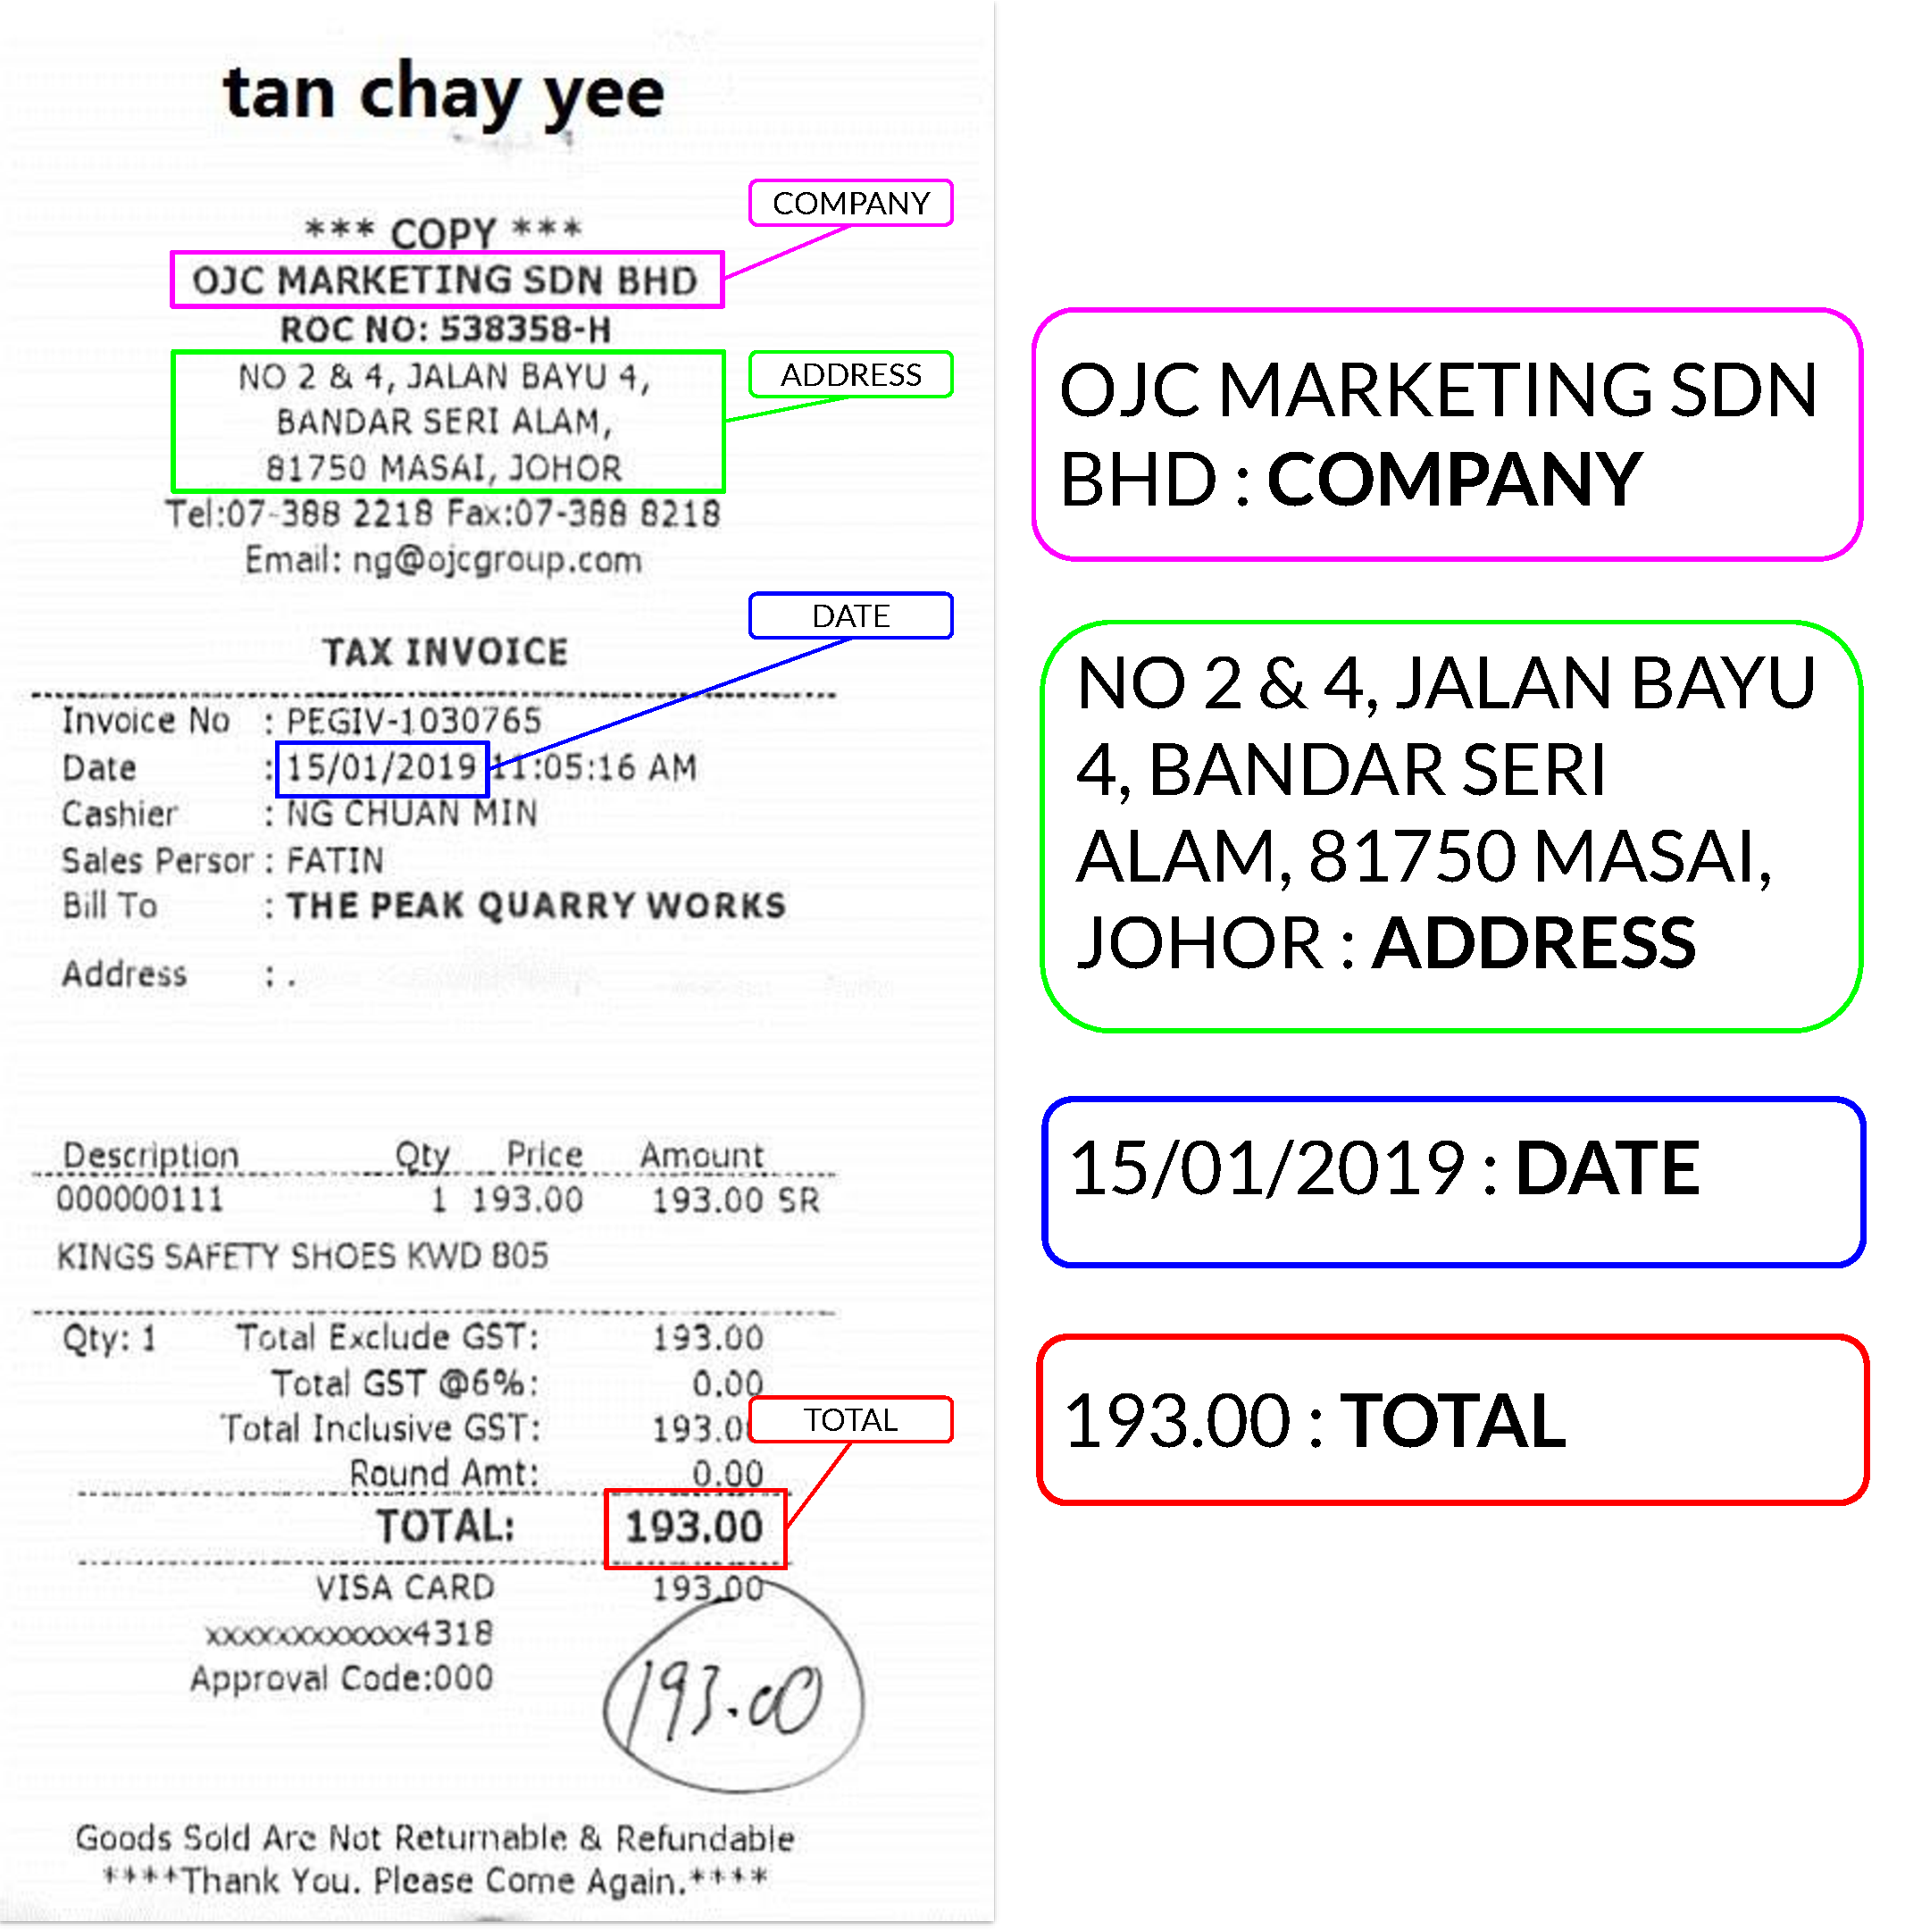
\includegraphics[width=\textwidth]{images/chapter4/sroie_sample_and_output.pdf}
    \caption{SROIE}
  \end{subfigure}
  \begin{subfigure}[b]{0.6\textwidth}
    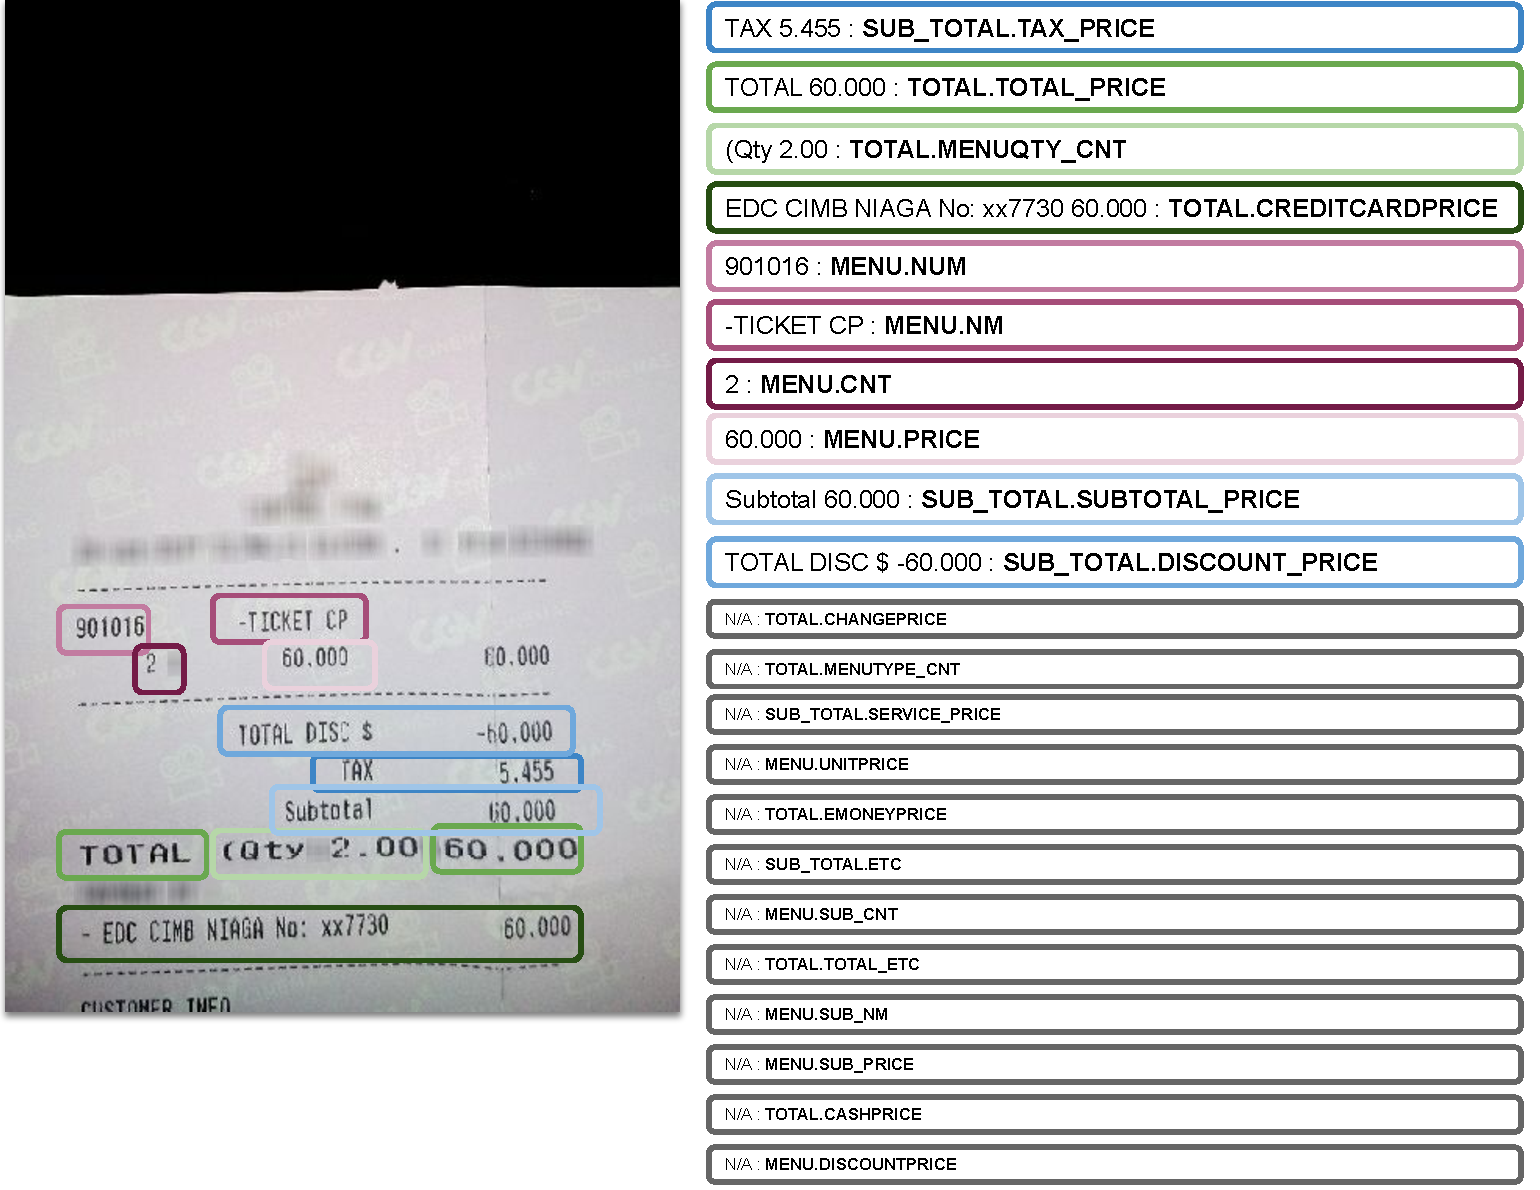
\includegraphics[width=\textwidth]{images/chapter4/cord_sample_and_output.pdf}
    \caption{CORD}
  \end{subfigure}
  \caption{Example document from FUNSD (a), SROIE (b), and CORD (c), accompanied by their corresponding target sequences that include the entities to be extracted paired with their corresponding keys.}
    \label{fig:source-target-sample}
\end{figure}

\subsection{Results and Discussion}

\subsubsection{Next Token Position Prediction}

\begin{table}
  \centering
  \small
  \begin{adjustbox}{max width=\textwidth}
  \begin{threeparttable}
  \begin{tabular}{cccc}
      \toprule
          Number of Layers & Pre-training Dataset & Accuracy \\ 
      \midrule
          1                & IIT-CDIP             & 67.10\%  \\
          1                & ReadingBank          & 89.37\%  \\
          2                & ReadingBank          & \textbf{95.86}\%   \\
      \bottomrule
  \end{tabular}
  \end{threeparttable}
  \end{adjustbox}
  \caption{Accuracy in predicting the next token for pairs sourced from ReadingBank, which were not used for pre-training. Selected pairs are considered "difficult", meaning that the tokens are positioned on different lines.}
  \label{table:next-token-prediction-results}
\end{table}

We evaluate the performance of the Layout2Pos module by computing the accuracy of next token position prediction on a set of pairs of consecutive tokens derived from 100 examples from ReadingBank, which were not used in the pre-training phase. Specifically, we curated pairs categorized as "difficult", where the tokens are positioned on different lines, making a raster-scan approach ineffective. This choice demands the model to leverage layout information to accurately predict the next token in these scenarios.

In these experiments, we exclusively train and evaluate Layout2Pos, omitting the encoder-decoder architecture. The accuracy for each token is determined by comparing the position of the ground-truth next token in the sequence with the position of the token corresponding to the maximum logit in the generated attention scores. We vary the number of layers and the pre-training dataset used. Performance is reported in Table~\ref{table:next-token-prediction-results}. Notably, pre-training Layout2Pos on ReadingBank compared to IIT-CDIP yields an increase of over 22\% in accuracy. Additionally, our results indicate that augmenting the number of layers in Layout2Pos results in a notable increase of over 6\% in accuracy. These results highlight the significance of using documents with accurate reading orders and contextualizing layout information to produce 1D position embeddings able to capture the reading order of documents.

\subsubsection{Visual Information Extraction}

% \begin{table}
%   \centering
%   \small
%   \begin{adjustbox}{max width=\textwidth}
%   \begin{threeparttable}
%   \begin{tabular}{llccccccccccc}
%       \toprule
%           % \textbf{Model}  & & \textbf{Prec.} & \textbf{Rec.} & \textbf{F1}  & \shortstack{\textbf{Hallucination} \\ \textbf{Rate}} & \shortstack{\textbf{Repetition} \\ \textbf{Rate}} & \shortstack{\textbf{Wrong Label} \\ \textbf{Rate}} & \shortstack{\textbf{Omission} \\ \textbf{Rate}} & \shortstack{\textbf{“Other"} \\ \textbf{Rate}} \\ 
%       %     \textbf{Model}  & & \textbf{Precision} & \textbf{Recall} & \textbf{F1}  & \rotatebox{-90}{\textbf{Hallucination Rate}} & \rotatebox{-90}{\textbf{Repetition Rate}} & \rotatebox{-90}{\textbf{Wrong Label Rate}} & \rotatebox{-90}{\textbf{Omission Rate}} & \rotatebox{-90}{\textbf{“Other” Rate}} \\
%        &   & & &  & &  \multicolumn{5}{c}{\textbf{Rate}} \\ 
%        \textbf{Dataset} & \textbf{Model} & \shortstack{\textbf{Filter out}\\\textbf{Repetitions}} & \textbf{Prec.} & \textbf{Rec.} &   \textbf{F1} & \rotatebox{-90}{\textbf{Hallucination}} & \rotatebox{-90}{\textbf{Repetition}} & \rotatebox{-90}{\textbf{Wrong Label}} & \rotatebox{-90}{\textbf{Omission}} & \rotatebox{-90}{\textbf{"Other"}} \\
%       \midrule
%       \multirow{4}{*}{FUNSD} & LayoutLM  \citep{xu2020layoutlm} & \cellcolor[gray]{0.9} & 75.91 & 80.54 &	78.16 & \cellcolor[gray]{0.9} & \cellcolor[gray]{0.9} & \cellcolor[gray]{0.9} & \cellcolor[gray]{0.9} &  \cellcolor[gray]{0.9} \\
%       & LayoutLMv2-no-visual             & \cellcolor[gray]{0.9} & 78.58 &	81.49 &	80.01 & \cellcolor[gray]{0.9} & \cellcolor[gray]{0.9} & \cellcolor[gray]{0.9} & \cellcolor[gray]{0.9} &  \cellcolor[gray]{0.9} \\  
%       & BART+2D & \xmark & 75.51	& 82.95 & 79.06 &  4.08 &	10.85 &	2.59 & 25.27 & 53.20 \\
%       & BART+2D & \cmark & 75.82 &	82.95 &	79.22 & 11.57 & 10.18 & 0.00 & 24.24 & 50.01 \\ 
%       & BART+Layout2Pos & \xmark & 75.34 & 82.84 &	78.91 & 3.26 &	18.59 &	1.72 &	27.69 &	42.74 \\
%       & BART+Layout2Pos & \cmark & 75.64 & 82.84 &	79.08 & 7.68 & 18.14 & 0.00 & 26.89 & 41.28 \\
%       \midrule
%       \multirow{4}{*}{SROIE} & LayoutLM  \citep{xu2020layoutlm} & \cellcolor[gray]{0.9} & 90.74 & 93.95 & 92.32 & \cellcolor[gray]{0.9} & \cellcolor[gray]{0.9} & \cellcolor[gray]{0.9} & \cellcolor[gray]{0.9} &  \cellcolor[gray]{0.9} \\ 
%       & LayoutLMv2-no-visual             & \cellcolor[gray]{0.9} & 93.20 &	93.88 &	93.54 & \cellcolor[gray]{0.9} & \cellcolor[gray]{0.9} & \cellcolor[gray]{0.9} & \cellcolor[gray]{0.9} &  \cellcolor[gray]{0.9} \\
%       & BART+2D & \xmark & 89.61 &	93.72 &	91.62 & 1.15 &	5.00 &	6.97 &	0.00 &	12.80 \\
%       & BART+2D & \cmark & 92.06 &	93.72 & 92.88 & 1.25 &	5.60 &	0.00 &	0.00 & 13.62 \\
%       & BART+Layout2Pos & \xmark & 88.99 &	92.91 &	90.91 & 2.38 &	6.03 &	3.12 &	0.24 &	14.17 \\
%       & BART+Layout2Pos & \cmark & 90.08 &	92.91 &	91.47 & 1.03 &	6.99 &	0.00 &	0.20 &	19.16 \\
%       \midrule
%       \multirow{4}{*}{CORD} & LayoutLM  \citep{xu2020layoutlm} & \cellcolor[gray]{0.9} & 93.91 & 95.11 & 94.51 & \cellcolor[gray]{0.9} & \cellcolor[gray]{0.9} & \cellcolor[gray]{0.9} & \cellcolor[gray]{0.9} &  \cellcolor[gray]{0.9} \\ 
%       & LayoutLMv2-no-visual             & \cellcolor[gray]{0.9} & 93.14 &	94.89 &	94.00 & \cellcolor[gray]{0.9} & \cellcolor[gray]{0.9} & \cellcolor[gray]{0.9} & \cellcolor[gray]{0.9} &  \cellcolor[gray]{0.9} \\  
%       & BART+2D & \xmark \\
%       & BART+Layout2Pos & \xmark \\
%       \bottomrule
%   \end{tabular}
%   \end{threeparttable}
%   \end{adjustbox}
%   \caption{Model performance (in \%) on FUNSD, SROIE, and CORD.}
%   \label{table:visual-information-extraction-results}
% \end{table}

\begin{table}
  \centering
  \small
  \begin{adjustbox}{max width=\textwidth}
  \begin{threeparttable}
  \begin{tabular}{llccccccccccc}
      \toprule
          % \textbf{Model}  & & \textbf{Prec.} & \textbf{Rec.} & \textbf{F1}  & \shortstack{\textbf{Hallucination} \\ \textbf{Rate}} & \shortstack{\textbf{Repetition} \\ \textbf{Rate}} & \shortstack{\textbf{Wrong Label} \\ \textbf{Rate}} & \shortstack{\textbf{Omission} \\ \textbf{Rate}} & \shortstack{\textbf{“Other"} \\ \textbf{Rate}} \\ 
      %     \textbf{Model}  & & \textbf{Precision} & \textbf{Recall} & \textbf{F1}  & \rotatebox{-90}{\textbf{Hallucination Rate}} & \rotatebox{-90}{\textbf{Repetition Rate}} & \rotatebox{-90}{\textbf{Wrong Label Rate}} & \rotatebox{-90}{\textbf{Omission Rate}} & \rotatebox{-90}{\textbf{“Other” Rate}} \\
       &   & & &  & &  \multicolumn{4}{c}{\textbf{Rate}} \\ 
       \textbf{Dataset} & \textbf{Model} & & \textbf{Prec.} & \textbf{Rec.} &   \textbf{F1} & \rotatebox{-90}{\textbf{Repetition}} & \rotatebox{-90}{\textbf{Hallucination}} & \rotatebox{-90}{\textbf{Wrong Label}} & \rotatebox{-90}{\textbf{Omission}} & \rotatebox{-90}{\textbf{Non-entity}} \\
      \midrule
      \multirow{4}{*}{FUNSD} & LayoutLM  \citep{xu2020layoutlm} & & 75.91 & 80.54 &	78.16 & \cellcolor[gray]{0.9} & \cellcolor[gray]{0.9} & \cellcolor[gray]{0.9} & \cellcolor[gray]{0.9} &  \cellcolor[gray]{0.9} \\
      & LayoutLMv2-no-visual             &  & 78.58 &	81.49 &	80.01 & \cellcolor[gray]{0.9} & \cellcolor[gray]{0.9} & \cellcolor[gray]{0.9} & \cellcolor[gray]{0.9} &  \cellcolor[gray]{0.9} \\  
      & BART+2D & & 77.89 &	82.10 &	79.94 &  2.09 & 1.65 &	41.38 &	42.79 &	6.09 \\ 
      & BART+Layout2Pos & & 79.65 & 78.30 &	78.97 &	2.25 & 	2.89 &	30.80 &	59.26  & 2.78  \\
      \midrule
      \multirow{4}{*}{SROIE} & LayoutLM  \citep{xu2020layoutlm} &  & 90.74 & 93.95 & 92.32 & \cellcolor[gray]{0.9} & \cellcolor[gray]{0.9} & \cellcolor[gray]{0.9} & \cellcolor[gray]{0.9} & \cellcolor[gray]{0.9} \\ 
      & LayoutLMv2-no-visual             &  & 93.20 &	93.88 &	\textbf{93.54} & \cellcolor[gray]{0.9} & \cellcolor[gray]{0.9} & \cellcolor[gray]{0.9} & \cellcolor[gray]{0.9} &  \cellcolor[gray]{0.9} \\
      & BART+2D & & 93.18 &	93.44 &	93.31 &	0.00 & 	0.14 &	0.00 &	17.46 &	3.43 \\
      & BART+Layout2Pos & & 92.78 &	93.52 &	93.15 & 0.00 &	0.24 &	0.29 &	17.29 & 3.22 \\
      \midrule
      \multirow{4}{*}{CORD} & LayoutLM  \citep{xu2020layoutlm} & & 93.91 & 95.11 & 94.51 & \cellcolor[gray]{0.9} & \cellcolor[gray]{0.9} & \cellcolor[gray]{0.9} & \cellcolor[gray]{0.9} & \cellcolor[gray]{0.9}  \\ 
      & LayoutLMv2-no-visual             & & 93.14 &	94.89 &	94.00 & \cellcolor[gray]{0.9} & \cellcolor[gray]{0.9} & \cellcolor[gray]{0.9} & \cellcolor[gray]{0.9} &  \cellcolor[gray]{0.9} \\  
      & BART+2D & & 94.32 & 92.41 &	93.35 & 1.36 & 0.00 &	6.27 &	25.19 & 0.19 \\
      & BART+Layout2Pos & & 95.42 &	93.91 &	\textbf{94.66} & 2.86 & 1.16 & 5.69 &	18.96 &	0.33 \\
      \bottomrule
  \end{tabular}
  \end{threeparttable}
  \end{adjustbox}
  \caption{Model performance (in \%) on FUNSD, SROIE, and CORD.}
  \label{table:visual-information-extraction-results}
\end{table}


Table~\ref{table:visual-information-extraction-results} reports the performance of all four models on FUNSD, SROIE, and CORD.


\section{Conclusion}